\documentclass[aps,prb,showpacs,longbibliography]{revtex4-1}
\usepackage{geometry}                
\geometry{letterpaper}                 
\usepackage{graphicx}
\usepackage{epsf,amsmath,amssymb,amsfonts}
\usepackage{amssymb,amsmath}
\usepackage{epstopdf}
\usepackage{pdfsync}

 \usepackage[colorlinks=true]{hyperref}
 \hypersetup{urlcolor=blue, citecolor=blue, linkcolor=blue}
\numberwithin{equation}{section}
\newcommand{\field}[1]{\mathbb{#1}}
\newtheorem{alg}{Algorithm}[section]
\newtheorem{thm}{Theorem}[section]
\newtheorem{lem}[thm]{Lemma}
\newtheorem{cor}[thm]{Corollary}
\newtheorem{pro}{Proposition}[section]
\newtheorem{defn}{Definition}[section]
\newtheorem{asp}{Assumption}[section]
\newtheorem{rmk}{Remark}[section]

\def\ds{\displaystyle}
\def\ni{\noindent}
\begin{document}

\title{Critical events, entropy, and 
the grain boundary character distribution}
 \author{K.~Barmak}
 \email{katayun@andrew.cmu.edu}
 \affiliation{Materials Research Science and Engineering Center\\Department of Materials Science
  and Engineering, Carnegie Mellon University, Pittsburgh, PA 15213}
  \author{E.~Eggeling}
  \email{eva.eggeling@fraunhofer.at}
  \affiliation{Fraunhofer Austria Research GmbH, Visual Computing, A-8010 Graz}
  \author{M.~Emelianenko}
  \email{memelian@gmu.edu}
  \affiliation{Department of Mathematics, George Mason University, Fairfax, VA 22030}
  \author{Y.~Epshteyn} 
  \email{epshteyn@math.utah.edu}
  \affiliation{Department of Mathematics, The University of Utah, Salt Lake City, UT 84112}
   \author{D.~Kinderlehrer}
   \email{davidk@andrew.cmu.edu}  
   \author{R.~Sharp}
   \email{rsharp@gmail.com}
   \author{S.~Ta'asan}
   \email{shlomo@andrew.cmu.edu}
\affiliation{Materials Research Science and Engineering Center\\Center for Nonlinear Analysis and Department of Mathematical Sciences, Carnegie
    Mellon University, Pittsburgh, PA 15213}

\begin{abstract} Mesoscale experiment and simulation permit harvesting information about both geometric features and texture in polycrystals.  The grain boundary character distribution (GBCD) is an empirical distribution of the relative length (in 2D) or area (in 3D) of interface with a given lattice misorientation and normal. During the growth process, an initially random distribution of boundary types reaches a steady state that is strongly correlated to the interfacial energy density.  In simulation, it is found that if the given energy density depends only on lattice misorientation, then the steady state GBCD and the energy are related by a Boltzmann distribution.   This is among the simplest non-random distributions, corresponding to independent trials with respect to the energy.

In this paper we derive an entropy based theory which suggests that the evolution of the GBCD  satisfies a Fokker-Planck Equation, an equation whose stationary state is a Boltzmann distribution.  Cellular structures coarsen according to a local evolution law, curvature driven growth, and are limited by space filling constraints.  The interaction between the evolution law and the constraints is governed primarily by the force balance at triple junctions, the natural boundary condition associated to curvature driven growth, and determines a dissipation relation.  A simplified coarsening model is introduced which is driven by the boundary conditions and reflects the network level dissipation relation of the grain growth system.  It resembles an ensemble of inertia-free spring-mass-dashpots.  Application is made of the recent characterization of Fokker-Planck kinetics as a gradient flow for a free energy in deriving the theory.  The theory predicts the results of large scale 2D simulations and is consistent with experiment.  
\end{abstract}
\pacs{61.72.Mm, 68.35.-p, 89.70.Cf, 05.70.Ln }
\maketitle
   \section{Introduction} Cellular networks are ubiquitous in nature.  They exhibit behavior on many different length and time scales and are generally metastable. Most technologically useful materials are 
  polycrystalline microstructures composed of a myriad of small
  monocrystalline grains separated by grain boundaries, and thus comprise cellular networks.  The
  energetics and connectivity of the grain boundary network plays a crucial role in determining the properties of a material across a wide range of scales.  A central problem in materials is to  develop technologies capable of producing an arrangement of grains that provides for a desired set of material
properties.  Traditionally the focus has been on the geometric feature of size and the preferred distribution of grain orientations, termed texture.  More recent mesoscale experiment and simulation permit harvesting large amounts of information about both geometric features and crystallography of the boundary network in material microstructures, \cite{ISI:000071740700001,dk:adams,ISI:000225119800166,ISI:000231321200007,ISI:000248758300020}


A leading candidate to characterize texture of the grain boundary population is the grain boundary character distribution\cite{ISI:000225119800166}.  The grain boundary character distribution (GBCD) is an empirical distribution of the relative length (in 2D) or area (in 3D) of interface with a given lattice misorientation and grain boundary normal. During the growth process, an initially random grain boundary texture reaches a steady state that is strongly correlated to the interfacial energy density.  In simulation, a GBCD is always found.  In our view, it is the GBCD which should serve as a reference distribution for texture in preference to other distributions.

 If the given energy depends only on lattice misorientation, then the steady state GBCD and the interfacial energy density are related by a Boltzmann distribution.   This is among the simplest non-random distributions, corresponding to independent trials with respect to the density.  It offers compelling evidence that the GBCD is a material property.  Why does such a simple distribution arise from such a complex system?

We outline a new entropy based theory which suggests that the evolving GBCD  satisfies a Fokker-Planck Equation.  Coarsening in polycrystalline systems is a complicated process involving details of material structures, chemistry, arrangement of grains in the configuration, and environment.  In this context, we consider just two competing global features, as articulated by C. S. Smith \cite{Smith:MI:1952}:  cell growth according to a local evolution law and space filling constraints.   We shall impose curvature driven growth for the local evolution law, cf. Mullins \cite{Mullins:MS:1963}.  Space filling requirements are managed by critical events, rearrangements of the network involving deletion of small contracting cells and facets.  The interaction between the evolution law and the constraints is, we shall discover, governed primarily by the balance of forces at triple junctions. This balance of forces, often referred to as the Herring Condition,\cite{Herring:PPM:1951} is the natural boundary condition associated with the equations of curvature driven growth. It determines a dissipation relation for the network as a whole.  

We introduce a simplified coarsening model driven by the boundary conditions that reflects the dissipation relation of the grain growth system.  It resembles an ensemble of inertia-free spring-mass-dashpots\footnote{See page 6\cite{MR823984}}.  For this simpler network, we learn how entropic or diffusive behavior at the large scale emerges from a dissipation relation at the scale of local evolution.  The cornerstone is our novel implementation of the iterative scheme for the Fokker-Planck Equation in terms of the system free energy and a Kantorovich-Rubinstein-Wasserstein metric \cite{ISI:000071938700001}, cf. also \cite{ISI:A1997YC73400019}, which will be defined and explained later in the text.  The network level nonequlibrium nature of the iterative scheme leaves free a temperature-like parameter.  The entropy method is exploited to identify uniquely this parameter. 
To illustrate the idea, we include a simple application to the solution of the Fokker-Planck Equation itself.  

We present evidence that the theory predicts the results of large scale 2D simulations \cite{DK:BEEEKT}.  
Energy densities consisting of quadratic and quartic trigonometric polynomials are analyzed in detail.  The discussion of the quartic based energy density places in relief the entropic nature of the GBCD.  It would take us rather far afield to discuss consistency with experiment and we refer to  \cite{ISI:000225119800166}.  A companion paper emphasizing the mathematical and simulation issues of the project is \cite{DK:gbtheory}.  A theory for the evolution of geometric features of microstructure is discussed in \cite{MR2223359,MR2581030}.  Some of the results of the present work were announced in \cite{dk:rexggIV, DK:BEEEKT}.  Different treatments of texture development are given in \cite{ISI:000272111800015, ISI:000272405600002} and \cite{ISI:000170652100012, ISI:000170428100003}.
\section{Mesoscale theory}  Our point of departure is the common denominator theory for the mesoscale description of grain growth.  This is curvature driven growth, more precisely the equation  (\ref{ME})  below, for the motion of curves or arcs individually or in a network, which we employ for our local law of evolution.  Boundary conditions must be imposed where the arcs meet.  This condition is the Herring Condition, (\ref{HC}),  which is the natural boundary condition at equilibrium for (\ref{ME}).   Since their appearance by Mullins for general or anisotropic growth, 
\cite{Mullins:MS:1963}, and Herring, \cite{Herring:PPM:1951, Herring:SPSS:1952}, 
a large and distinguished body of work has grown about these equations.  Most relevant to here are 
\cite{DKgurtin, MR1240580,ISI:000169336700007, ISI:A1988P835300016}.  
Let  $\alpha$  denote the misorientation between two grains separated by an arc  $\Gamma$, as noted in FIG.~\ref{fig:curve},   with normal  $n = (\cos \theta, \sin \theta)$, tangent direction  $b$  and curvature  $\kappa$.  Let  $\psi = \psi(\theta,\alpha)$  denote the energy density on  $\Gamma$.  So, representing the time evolving arc  $\Gamma$  in the  $x = (x_1,x_2)$  plane by the vector valued function  $\xi(s,t) = (\xi_1(s,t),\xi_2(s,t))$  of arc parameter  $s$  and time  $t$,
\begin{equation}
\Gamma:  x = \xi(s,t), \ \ 0 \leqq s \leqq L, \ t > 0,
\end{equation}
with
\begin{equation*} \begin{aligned}  b = \frac{\partial \xi}{\partial s} \ & \textrm{(tangent)}, \ \  n = Rb \ \textrm{(normal),} \\
v = \frac{\partial \xi}{\partial t} \  & \textrm{(velocity),} \ v_n = v \cdot n  \textrm{(normal velocity)}
\end{aligned}
\end{equation*}
where  $R$  is a positive rotation of  $\pi/2$.  The Mullins Equation of evolution is
\begin{equation} \label{ME}
v_n = (\psi_{\theta \theta} + \psi) \kappa \ \textrm{on} \ \Gamma.
\end{equation} 
\begin{figure}[htbp] 
   \centering
    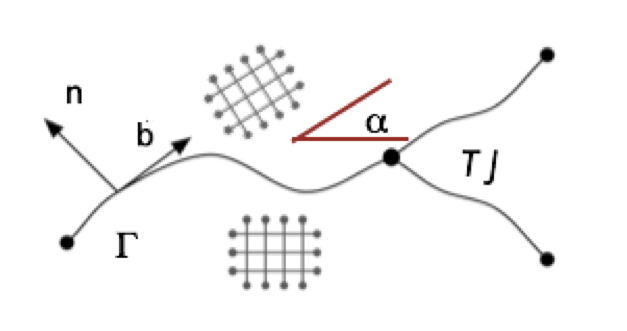
\includegraphics[width=2.25in]{fig_1.eps} 

   \caption{ \label{fig:curve} (Color online) An arc  $\Gamma$  with normal  $n$, tangent $b$, and lattice misorientation  $\alpha,$  illustrating lattice elements.(reproduced from \cite{dk:rexggIV})}
\end{figure}

We assume that only triple junctions are stable and that the Herring Condition holds at triple junctions.  This means that whenever three curves $\{ \Gamma^{(1)}, \Gamma^{(2)}, \Gamma^{(3)} \}$   meet at a point  $p$ the force balance, (\ref{HC}) below, holds:
\begin{equation} \label{HC}
\sum_{i = 1,..,3} (\psi_\theta n^{(i)} + \psi b^{(i)})  =  0.
\end{equation}
It is easy to check, \cite{ISI:000169336700007}, that the instantaneous rate of change of energy of  $\Gamma$  is
\begin{equation} \label{en1}
\frac{d}{dt} \int_\Gamma \psi |b| ds  =  - \int_\Gamma v_n^2 ds + v
\cdot (\psi_\theta n + \psi b) |_{\partial \Gamma}
\end{equation}
We turn now to a network of grains bounded by a collection of curves  $\{ \Gamma_i \}$  subject to some condition at the border of the region they occupy, like fixed end points or periodicity, cf. FIG.~\ref{fig:network}.  
\begin{figure}[htbp] 
   \centering
   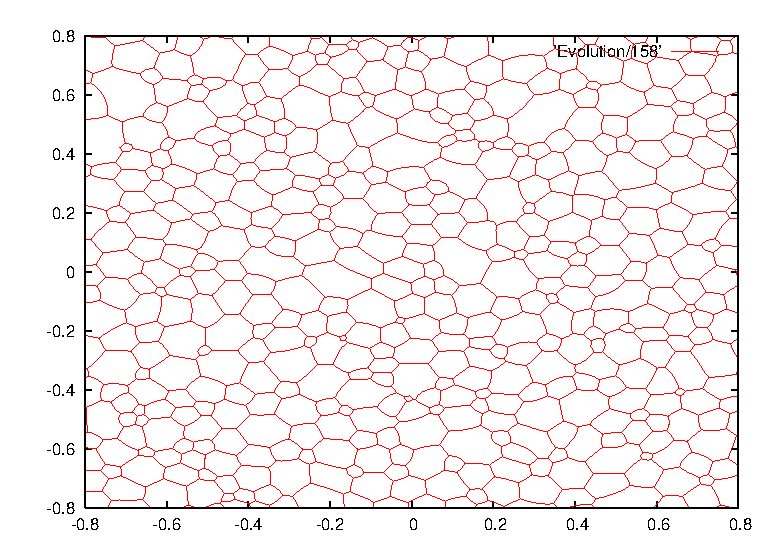
\includegraphics[width=3in, height = 3.12in]{fig_2.eps} 
   \caption{ \label{fig:network}(Color online) Example of an instant during the simulated evolution of a cellular network.  This is part of the frame from a small simulation with constant energy density and periodic conditions at the border of the configuration.}
\end{figure}
Our simulation is described in \cite{ISI:000242573400006, ISI:000225119800165}.  The typical simulation consists in initializing a configuration of cells and their boundary arcs, usually by a modified Voronoi tessellation, assigning random orientations to the cells, and then solving the system (\ref{ME}), (\ref{HC}), eliminating facets when they have negligible length and cells when they have negligible area.  The simulation satisfies all known diagnostics and, in particular, when  $\psi =$ constant, the von Neumann-Mullins $n-6$ rule\cite{vonNeumann:MI:1952,Mullins:JAP:1956} is satisfied for each cell at each time when it is not subjected to a critical event, facet or grain deletion.

The total energy of the system is given by 

\begin{equation} \label{en2}
E(t)  =  \sum_{\{\Gamma_i\}} \int_{\Gamma_i} \psi |b| ds
\end{equation}
Owing exactly to the Herring Condition (\ref{HC}), the instantaneous rate of change of the energy
\begin{equation} \label{en3}
\begin{aligned}
\frac{d}{dt} E(t)  = & - \sum_{\{\Gamma_i\}} \int_{\Gamma_i}  v_n^2 ds  + \sum_{TJ} v \cdot \sum (\psi_\theta n + \psi b) \\
= & - \sum_{\{\Gamma_i\} } \int_{\Gamma_i} v_n^2 ds \\
\leqq & \ 0,
\end{aligned}
\end{equation}
rendering the network dissipative for the energy in any instant absent of critical events.  Indeed, in an interval $(t_0, t_0 + \tau)$ where there are no critical events, we may integrate  (\ref{en3})  to obtain a local dissipation equation
\begin{equation} \label{GBlocdis}
\sum_{\{\Gamma_i\}}\int_{t_0}^{t_0+\tau}\int_{\Gamma_i} v_n^2 dsdt + E(t_0 + \tau) = E(t_0)
\end{equation}
which bears a resemblance to the simple dissipation relation for an ensemble of inertia free springs with friction.  In the simulation, the facet interchange and cell deletion are arranged so that the inequality in  (\ref{en3})  is maintained.
In the case that the energy density is independent of the normal direction, so  $\psi = \psi(\alpha)$, the situation that will concern us in this paper,  (\ref{ME})  and  (\ref{HC})  may be expressed
\begin{eqnarray} 
v_n &=& \psi \kappa  \ \textrm{on} \ \Gamma \\
 \sum_{i = 1,...,3} \psi b^{(i)} &=& 0 \ \textrm{at} \ p, \label{ME2}
\end{eqnarray}
where  $p$  denotes a triple junction.  (\ref{ME2})  is the same as the Young wetting law\footnote{That is, the special case of (\ref{HC})\cite{Herring:PPM:1951,Herring:SPSS:1952}  when the interfacial energy density is independent of the normal direction, cf.\cite{dk:ohring}}.  Our interfacial energy densities  $\psi$  are chosen so that
\begin{equation} \label{rangepsi}  1 \leqq \psi(\alpha) \leqq \frac{3}{2}, \ |\alpha| \leqq \frac{\pi}{4}, \end{equation}
(periodic with period  $\pi/2$) giving square symmetry which is intended to mimic cubic symmetry in three dimensions.  For the range of  $\psi$  in (\ref{rangepsi}), one may check that  (\ref{ME2})  can always be resolved, namely, given three numbers  $\psi_i \in [1, 3/2]$  there are unit vectors  $b_i$  such that
$$ \psi_1 b_1 + \psi_2 b_2 + \psi_3 b_3 = 0.$$
In executing this check, one may note that if the oscillation in  $\psi$  is too large, then it may not be possible to fulfill the Young Law condition in general, cf.\cite{dk:adams} for a discussion of the issue.   
To develop the GBCD, the collection of misorientations must be sufficiently random, since for this type of density, all misorientations are drawn from initial list of pairwise differences of cell orientations.\footnote{Perhaps it is also of value to point out, in this context, that the failure of all but one cell to evacuate the network under  (\ref{rangepsi})  cannot be attributed 
to inability to form a triple junction but is likely due to configurational hinderance or near equilibrium behavior.}

For this situation we define the grain boundary character distribution, GBCD, with  $\Omega = (-\frac{\pi}{4},\frac{\pi}{4}],$
\begin{equation} \label{GBCD} \begin{aligned}
&\rho(\alpha,t) = \textrm{relative length of arc of misorientation} \\ & \alpha \ \textrm{at time} \ t ,
 \textrm{normalized so that} \\ 
&\ \ \ \  \int_\Omega \rho d\alpha = 1.
\end{aligned}
\end{equation}

\section{Simplified coarsening model}  A significant difficulty in developing a theory for the GBCD, and understanding texture development in general, lies in the lack of understanding of consequences of rearrangement events or critical events, facet interchange and grain deletion, on  misorientations and grain size.  For example, in FIG.~\ref{fig:5sides}, the average area of six-faceted grains during a growth experiment on an $Al$ thin film and the average area of six-faceted cells in a typical simulation both increase with time.  Note that the von Neumann-Mullins Rule is that the area  $A_n$  of a cell with  n-facets satisfies
\begin{equation} \label{n-6} A_n'(t)  =  c(n-6), \end{equation}
when  $\psi = const.$  and triple junctions meet at angles of  $2\pi/3$.  This is thought to hold approximately when anisotropy is small.  The von Neumann-Mullins Rule does not fail in the examples cited, of course, but cells observed at later times had 7, 8, ... facets at earlier times.  The trend of increase in average area over time holds for all facet classes.  Thus in the network setting, critical events and subsequent rearrangement play a major role.  Although we may be reasonably confident that small cells with  small numbers of facets will be deleted, their resulting effect on the configuration appears to be essentially random.  
\begin{figure}[htbp] 
   \centering
   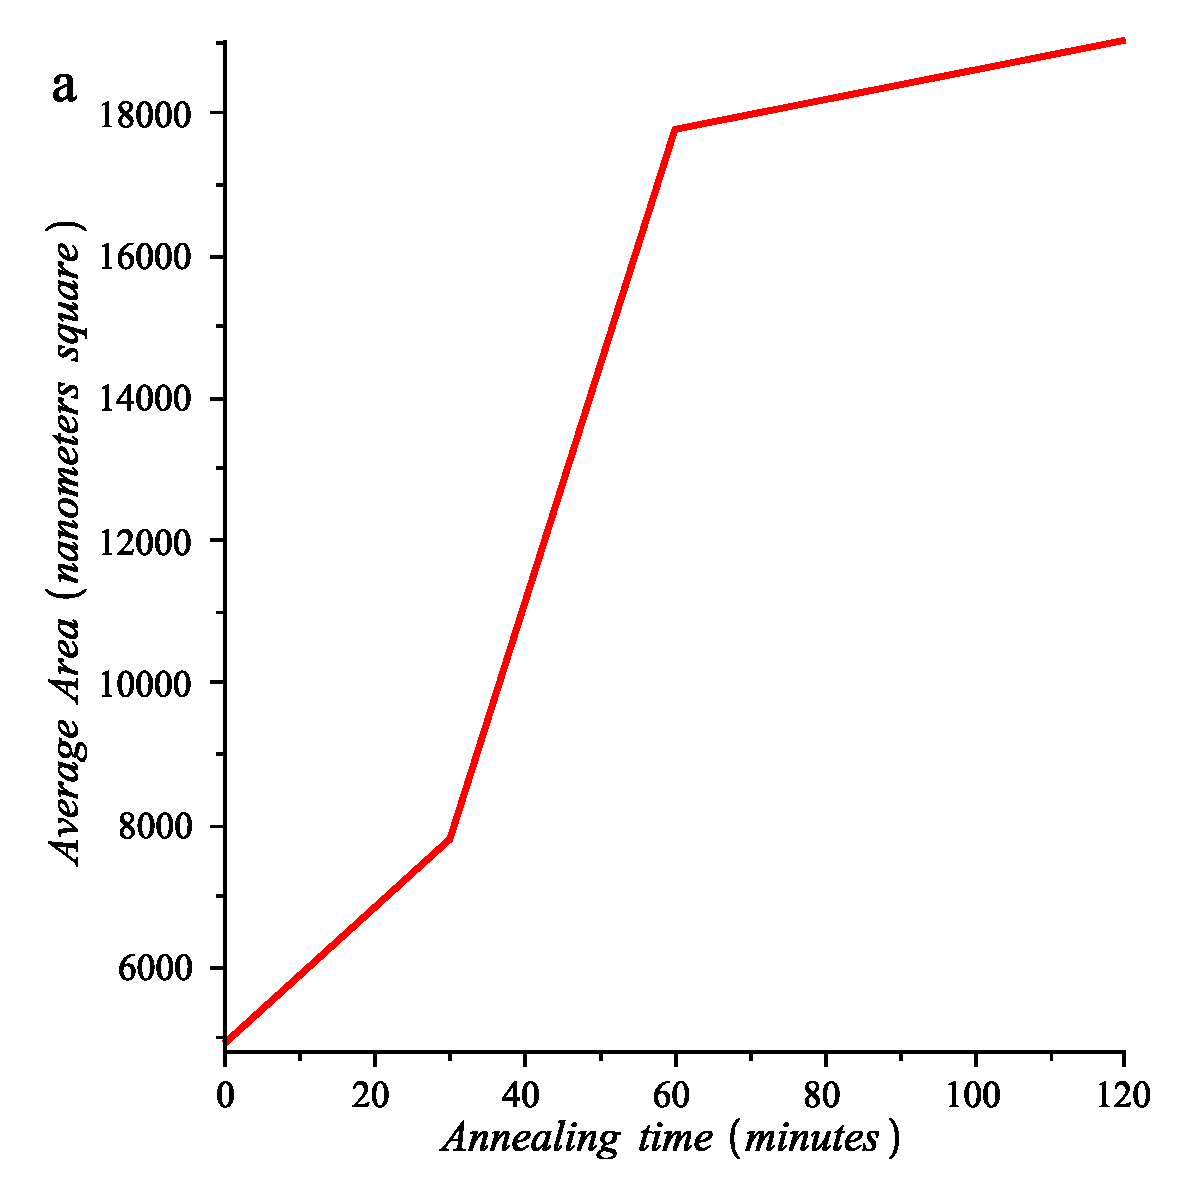
\includegraphics[width=2.5in]{fig_3a.eps} 
    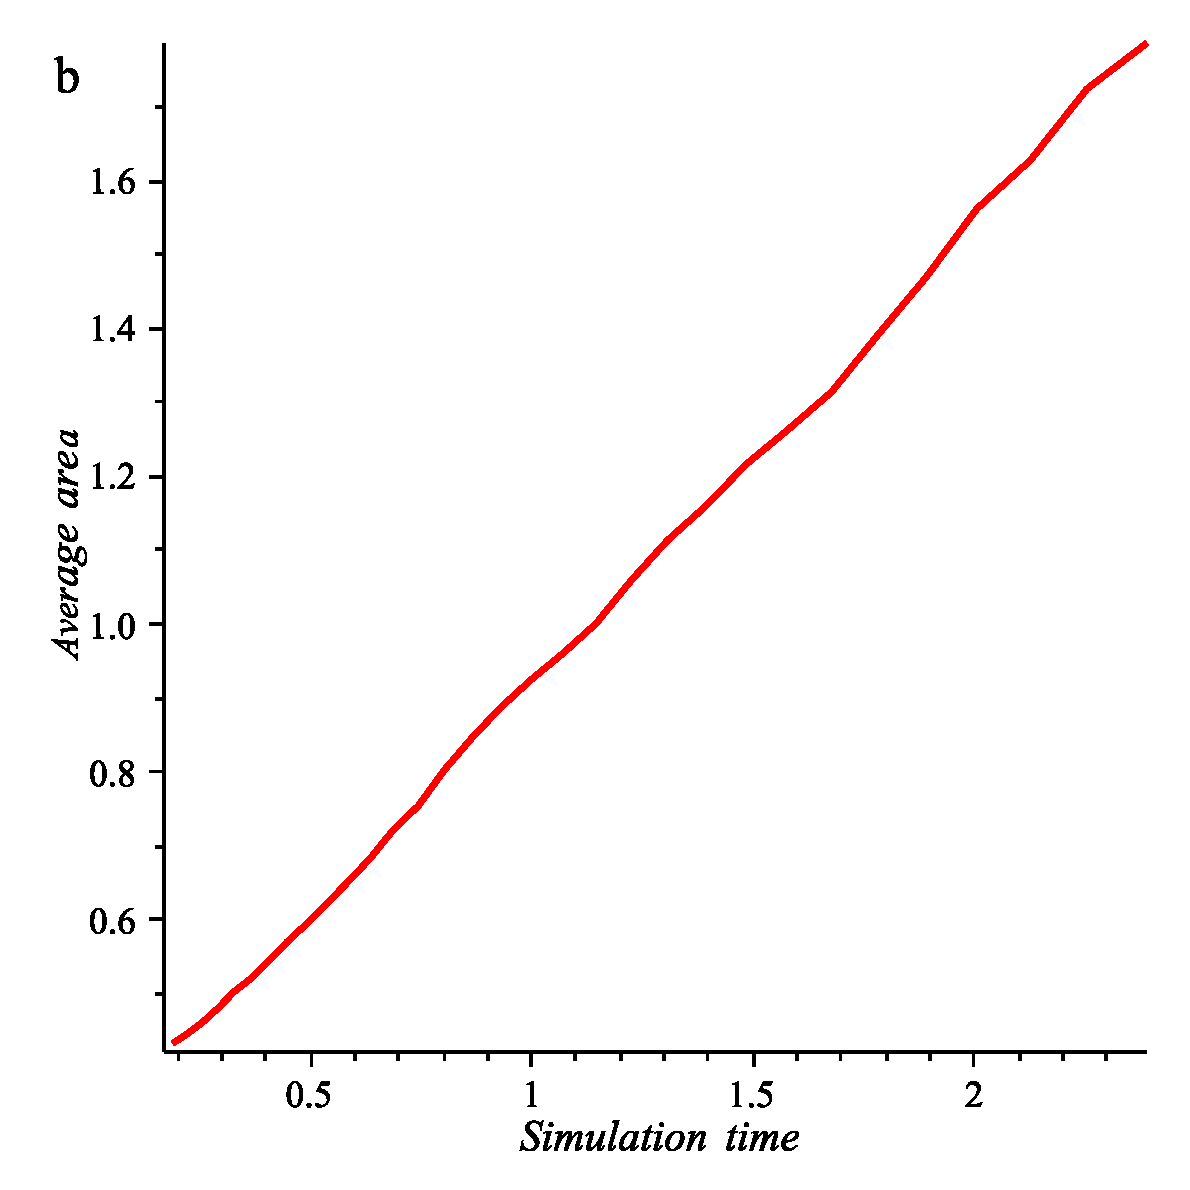
\includegraphics[width=2.5in]{fig_3b.eps} 
   \caption{ \label{fig:5sides}(Color online) The average area of six-sided cell populations during coarsening in two different cellular systems showing that the von Neumann-Mullins $n-6$-Rule (\ref{n-6}) does not hold at the scale of the network.  (a)  In an experiment on  $Al$ thin film\cite{DK:barmak} and  (b)  a typical simulation (arbitrary units).  }
\end{figure}


We shall study this by a simplified model which retains critical events and kinetics but neglects curvature driven motion of the boundaries.  It is an abstraction of the role of triple junctions in the presence of the rearrangement events.  We have used this model to develop a statistical theory for critical events, \cite{Barmak:2007vn, ISI:000260367300007, DK:BEGKT1}.  It has been found to have its own GBCD which we shall now study.  

Our theme will be that the GBCD statistic for the simplified model resembles the solution of a Fokker-Planck Equation obtained via the mass transport implicit scheme. The first part of the discussion consists in introducing this model.  The simplified model is formulated as a gradient flow which results in a dissipation inequality analogous to the one found for the coarsening grain network.  Because of this simplicity, it will be possible to `upscale' the network level system description to a higher level GBCD description that accomodates irreversibility.  As this changes the ensemble, following Boltzmann, there is an entropic contribution, which we take in the form of configurational entropy.  A more useful dissipation inequality is obtained by modifying the `velocity' term to be a true viscous term, which now brings us to the realm of the Kantorovich-Rubinstein-Wasserstein implicit scheme, sometimes referred to as the JKO-scheme.  At this stage, we explain how we may appeal to the Fokker-Planck paradigm.

The second part of the discussion, in section \ref{validation}, will be our argument to validate this paradigm.   We do not know that the statistic solves the Fokker-Planck PDE but we ask if it shares important aspects of Fokker-Planck behavior.  A defining characteristic of the Fokker-Planck Equation, and diffusion equations in general, is the exponential decay of their solutions to equilibrium.  We give evidence for this by asking for the unique `temperature-like' parameter that minimizes the relative entropy over long time.  The empirical stationary distribution and Boltzmann distribution with the special value of parameter are in excellent agreement, FIG.~ \ref{fig:OUsimp}.  This gives an explanation for the stationary distribution and the kinetics of evolution.
We do not know, at this point of our investigations, that the two dimensional network has the detailed dissipative structure of the simplified model, but we are able to produce evidence that the same argument employing the relative entropy does suggest the correct kinetics and stationary distribution.


\subsection{Formulation}  Let  $I \subset \textbf{R} $  be an interval of length  $L$   partitioned by points  $x_i, i = 1, \dots ,n$, where $x_i < x_{i+1}, i = 1, \dots ,n-1$  and  $x_{n+1}$ is identified with  $x_1$. For each interval  $[x_i,x_{i+1}], i = 1,\dots ,n,$  select a random misorientation number  $\alpha_i \in  (-\pi/4,\pi/4]$.  The intervals  $[x_i,x_{i+1}]$  correspond to grain boundaries with misorientations  $\alpha_i$  and the points  $x_i$  represent the triple junctions.   Choose an energy density  $\psi(\alpha) \geqq 0$  and introduce the energy
\begin{equation} \label{SME}
E = \sum_{i = 1,\dots,n} \psi(\alpha_i)(x_{i+1} - x_i).
\end{equation}
We impose gradient flow kinetics with respect to  (\ref{SME}), which is the system of ordinary differential equations
\begin{equation} \label{gflow} \begin{aligned}
& \frac{dx_i}{dt} = -\frac{\partial E}{\partial x_i}, i = 1,...,n, \ \textrm{that is } \\
& \frac{dx_i}{dt} = \psi(\alpha_{i}) - \psi(\alpha_{i-1}), i = 2...n, \ \textrm{and} \\ 
&\frac{dx_1}{dt} = \psi(\alpha_{1}) - \psi(\alpha_n)   .                          
\end{aligned} \end{equation}
The velocity  $v_i$  of the   $i^{th}$ boundary is
\begin{equation} \label{vel}
v_i = \frac{dx_{i+1}}{dt} - \frac{dx_i}{dt} = \psi(\alpha_{i-1}) - 2\psi(\alpha_i) + \psi(\alpha_{i+1}).
\end{equation}
The grain boundary velocities are constant until one of the boundaries collapses.  That segment is removed from the inventory of active cells and the velocities of its two neighbors are changed due to the emergence of a new junction.  Each such deletion event rearranges the network and, therefore, affects its subsequent evolution just as in the two dimensional cellular network.  Actually, since the interval velocities are constant, this gradient flow is just a sorting problem.  At any time, the next deletion event occurs at smallest of
$$ \frac{x_i -x_{i+1}}{v_i} \ \textrm{with} \ v_i < 0.$$

We turn to the dissipation inequality for the gradient flow.  At any time  $t$  between deletion events,
\begin{equation} \begin{aligned} \label{gfdiss}
\frac{dE}{dt}  &=  \sum \psi(\alpha_i) v_i \\
&= - \sum(\psi(\alpha_{i}) - \psi(\alpha_{i-1}))^2 \\
&= - \sum \frac{dx_i}{dt}^2 \leqq 0.
\end{aligned} 
\end{equation}


We may write a mass-spring-dashpot-like local dissipation inequality analogous to the grain growth one.  In an interval  $(t_0, t_0 + \tau)$  where there are no critical events,  $dE/dt$  may be integrated to give
$$
\tau \sum_{i = 1...n} \frac{dx_i}{dt}^2   +  E(t_0 + \tau)  = E(t_0)
$$
or
\begin{equation} \label{gflocdis}
\sum_{i = 1...n} \int_0^\tau \frac{dx_i}{dt}^2 dt  +  E(t_0 + \tau)  = E(t_0)
\end{equation}
With appropriate interpretation of the sum,  (\ref{gflocdis})  holds for all  $t_0$  and almost every  $\tau$  sufficiently small.  With the obvious use of Young's Inequality\footnote{$ \ 2ab \leqq a^2 + b^2$}, we have that
\begin{equation} \label{gflocdis2}
\frac{1}{4} \sum_{i = 1...n} \int_0^\tau v_i^2 dt  +  E(t_0 + \tau)  \leqq E(t_0)
\end{equation}
The energy of the system at time  $t_0 + \tau$  is determined by its state at time  $t_0$.  Vice versa, changing the sign on the right hand side of  (\ref{gflow})  allows us to begin with the state at time  $t_0+\tau$  and return to the state of time  $t_0$:  the system is reversible in an interval of time absent of rearragement events.  This is no longer the situation after such an event.  At the later time, we have no knowledge about which interval, now no longer in the inventory, was deleted.  

We introduce a new ensemble based on the misorientation parameter  $\alpha$  where we take $\Omega:  -\frac{\pi}{4} \leqq \alpha \leqq \frac{\pi}{4},$  for later ease of comparison with the two dimensional network.  The $GBCD$  or character distribution in this context is, as expected, the histogram of lengths of intervals sorted by misorientation  $\alpha$  scaled to be a probability distribution on  $\Omega.$  To be precise, let
\begin{equation*} \begin{aligned} l_i(\alpha,t)  =&  \ x_{i+1}(t) - x_i(t)\\  = & \  \textrm{length of the  $i^{th}$  interval,} \\ & \ \textrm{where explicit note has been taken of} \\ & \ \textrm{its misorientation parameter} \  \alpha  \end{aligned} \end{equation*}  Now partition  $\Omega$  into  $m$ subintervals of length  $h = \frac{\pi}{2}  \frac{1}{m}$  and let
\begin{equation}  \begin{aligned} \label{gfGBCD}
& \rho(\alpha,t) = \sum_{\alpha'  \in ((k-1)h,kh]}  l_i(\alpha',t) \cdot \frac{1}{Lh}, \\ & \ \ \textrm{for} \ (k-1)h < \alpha \leqq kh, \ t > 0.
\end{aligned} \end{equation}
For this definition of the statistic,
$$ \int_\Omega \rho(\alpha,t) d\alpha = 1 $$
Note that
\begin{equation} \begin{aligned} \label{rhot}
& \frac{\partial \rho}{\partial t}(\alpha,t) = \sum_{\alpha' \in ((k-1)h,kh]} v_i(\alpha') \cdot \frac{1}{Lh}, \\
& \ \ \textrm{for} \ (k-1)h < \alpha \leqq kh.
\end{aligned}\end{equation}


We may express  (\ref{gflocdis2})  in terms of the character distribution  (\ref{gfGBCD}), which amounts to
\begin{equation} \label{gfGBCDloc} \begin{aligned}
& \mu_0 \int_{t_0} ^{t_0 + \tau} \int_\Omega |\frac{\partial \rho}{\partial t}|^2 d\alpha dt + \int_\Omega \psi(\alpha) \rho(\alpha,t_0+\tau)d\alpha  \\& \ \ \ \leqq \int_\Omega \psi(\alpha) \rho(\alpha,t_0) d\alpha,
\end{aligned} \end{equation}
where  $\mu_0 > 0$  is some constant.  

We now impose a modeling assumption.  The expression (\ref{gfGBCDloc})  is in terms of the new misorientation level ensemble, upscaled from the local level of the original system.  Consistent with the lack of reversibility when rearrangement events occur, an entropic term will be added.  We use standard configurational entropy,
\begin{equation} \label{entropy}
+ \int_\Omega \rho \log \rho d\alpha,
\end{equation}
although this is not the only choice.  
Minimizing  (\ref{entropy})  favors the uniform state, which would be the situation were  $\psi(\alpha) = $ constant.

Given that  (\ref{gfGBCDloc})  holds, we assume that for any  $t_0$  and  $\tau$  sufficiently small that
\begin{equation} \label{Ddis} \begin{aligned}
&\mu_0 \int_{t_0}^{t_0+\tau} \int_\Omega( \frac{\partial \rho}{\partial t})^2 d\alpha dt + \\ & \int_\Omega(\psi\rho + \lambda \rho\log \rho) d\alpha \vert_{t_0 + \tau} \\ & \ \ \ \ \  \leqq  \int_\Omega ( \psi \rho  +  \lambda  \rho \log \rho) d\alpha \vert_{t_0}.
\end{aligned} \end{equation}
$E(t)$  was analogous to an internal energy or the energy of a microcanonical ensemble and now  
\begin{equation} \label{F}  F(\rho)  =  F_\lambda(\rho)  =  E(t) + \lambda \int_\Omega \rho \log \rho d\alpha 
 \end{equation}
is a free energy.  

\subsection{Fokker Planck paradigm}  (\ref{Ddis}) above fails as a proper dissipation principle because the first term does not represent lost energy due to frictional or viscous forces.  For a deformation path  $f(\alpha,t), t_0 \leqq t \leqq t_0 + \tau,$  of probability densities, this quantity is
\begin{equation} \label{D}
D = D(f) = \int_0^\tau \int_\Omega v^2 f d\alpha dt
\end{equation}
where  $f,v$  are related by the continuity equation and initial and terminal conditions
\begin{equation} \label{conteqn} \begin{aligned}
& f_t + (vf)_\alpha = 0 \ \textrm{in} \ \Omega \times (t_0,t_0+\tau), \textrm{and} \\
& f(\alpha,t_0) = \rho(\alpha,t_0),  \ f(\alpha,t_0+\tau) = \rho(\alpha,t_0+\tau) \ \textrm{in} \ \Omega,
\end{aligned} \end{equation}
by analogy with fluids \cite{MR0108121}, p.53 et seq. and elementary mechanics.  

For brevity, set  $\rho^\ast(\cdot) = \rho(\cdot,t_0)$.  Our question now is whether or not the first term of   (\ref{Ddis})  can dominate the term  $D(f)$  for some  $f$  so that  $D(f)$  may be substituted while maintaining the inequality.  Using the deformation path given by  $\rho$  itself, we may calculate that indeed
\begin{equation} \begin{aligned} \label{D2}
D(\rho) & =  \int_0^\tau \int_\Omega v^2 \rho d\alpha dt \\ & \leqq \frac{c_\Omega}{\min_\Omega \rho} \cdot \int_0^\tau\int_\Omega (\frac{\partial \rho}{\partial t})^2 d\alpha dt,
\end{aligned} \end{equation}
where the  $v$  is chosen by solving explicitly the continuity equation  (\ref{conteqn}).  We now have that for any relaxation time  $\tau > 0$,
\begin{equation} \label{D3}
\frac{\mu}{2}  \int_0^\tau \int_\Omega v^2 \rho d\alpha dt+ F_\lambda(\rho) \leqq F_\lambda(\rho^\ast)
\end{equation}
for some constant  $\mu$.

The infimum of  $D(f)$  over all admissible  $(v,f)$  is a known statistical measure of closeness of probability densities, the square of the Kantorovich-Rubinstein-Wasserstein or Wasserstein metric. \cite{MR2401600, MR1964483}  For densities  $\rho,\rho^\ast$  it is defined to be
\begin{equation} \label{D4} \begin{aligned}
& d(\rho,\rho^\ast)^2  =  \inf_P \int_\Omega \int_\Omega |x - y|^2 dp(x,y) \\
& P = \textrm{joint distributions for} \ \rho,\rho^\ast \ \textrm{on} \ \bar{\Omega}\times \bar{\Omega},
\end{aligned}
\end{equation} 
Recall here that the probability density  $p(x,y)$  is a joint distribution for the probability distributions  $P$  and  $P^\ast$  with densities  $\rho$  and  $\rho^\ast$  provided that
\begin{equation*} \begin{aligned}
& P(E)  =  \int_E \rho(x) dx =  \int_E \int_\Omega dp(x,y) \ \textrm{and} \\
&P^\ast(F) =  \int_F \rho^\ast(y)dy = \int_\Omega \int_F dp(x,y) \\ & \ \ \ \ \ \textrm{for all} \ E,F \subset \Omega.
\end{aligned}
\end{equation*}
The metric  $d$ has the property that
\begin{equation} \label{D5}
\frac{1}{\tau}d(\rho,\rho^\ast)^2 = \inf D(f),
\end{equation}
where the infimum is taken over all deformation paths  $(f,v)$  satisfying  (\ref{conteqn}).\cite{MR1738163}  We next replace  (\ref{D3})  by a minimum principle, arguing that the path given by  $\rho(\alpha,t)$  is the one most likely to occur and that the minimizing path has the highest probability.
We are led to the variational principle for the unknown  $\rho$  given  $\rho^\ast$
\begin{equation} \label{D51}
\frac{\mu}{2\tau} d(\rho,\rho^\ast)^2 + F_\lambda(\rho) = \inf_{\{\eta\}}\{\frac{\mu}{2\tau} d(\eta,\rho^\ast)^2 + F_\lambda(\eta)\}.
\end{equation}
For each relaxation time  $\tau > 0$  we determine iteratively the sequence  $\{ \rho^{(k)} \} $  by choosing  $ \rho^\ast = \rho^{(k-1)}$  and  $\rho^{(k)} = \rho $  in (\ref{D51}) and set
\begin{equation} \label{D6}
\rho^{(\tau)}(\alpha,t) = \rho^{(k)}(\alpha)  \ \textrm{in} \ \Omega \ \textrm{for} \ k\tau \leqq t  < (k+1)\tau.
\end{equation}
We then anticipate recovering the GBCD  $\rho$ as
\begin{equation} \label{D7}
\rho(\alpha,t)  =  \lim_{\tau \rightarrow 0} \rho^{(\tau)}(\alpha,t),
\end{equation}
with the limit taken in a suitable sense.\footnote{Iterative schemes are among the most common ways of solving differential equations.  Generally they consist of metrics in competition with functionals.  The best known method for solving the diffusion equation, the backward Euler or implicit finite difference scheme \cite{MR1512478, MR827497}, is based on the variational principle for the unknown  $u$  given  $u^\ast$:
$$ \frac{1}{2\tau} \int_\Omega |u - u^*|^2 dx + \frac{k}{2} \int_\Omega |\nabla u|^2 dx = \min,$$
the  $L^2$  metric in competition with the Dirichlet Integral.
For each relaxation time  $\tau > 0$ determine the sequence  $\{ u^k \}$ by choosing  $ u^\ast = u^{(k-1)}$  and  $u = u^{(k)}$  in the variational principle above.  Then define  $u^{(\tau)}$ by
$$ u^{(\tau)}(x,t) =  u^{(k)}(x) \ \textrm{in} \ \Omega, \ k\tau \leqq  t < (k+1)\tau,$$
and let
$$ u = \lim_{\tau \rightarrow 0} u^{(\tau)}$$
Then  $u$  is a solution of the diffusion equation
$$ \frac{\partial u}{\partial t} = k \Delta u  \ \textrm{in} \ \Omega.  $$}
It has been recently established that  $\rho$  obtained from  (\ref{D7})  is the solution of the Fokker-Planck Equation\cite{ISI:000071938700001}
\begin{equation} \label{FP}
\mu \frac{\partial \rho}{\partial t} = \frac{\partial}{\partial \alpha}(\lambda \frac{\partial \rho}{\partial \alpha} + \psi' \rho) \ \textrm{in} \ \Omega, 0 < t < \infty.
\end{equation}
We might point out here, as well, that a solution of  (\ref{FP})  with periodic boundary conditions and nonnegative initial data is positive for  $t > 0$.
\section{Validation of the scheme} \label{validation} We now begin the validation step of our model. First we review a few facts about solutions of  (\ref{FP}).  Introduce the notation for the Boltzmann distribution with parameter  $\lambda$
\begin{equation}\begin{aligned}  \label{bol}
& \rho_\lambda(\alpha) = \frac{1}{Z_\lambda} e^{-\frac{1}{\lambda}\psi(\alpha)}, \alpha \in \Omega, 
\ \textrm{where} \\ & Z_\lambda = \int_\Omega 
e^{-\frac{1}{\lambda}\psi(\alpha)} d\alpha.
\end{aligned} \end{equation}
The Kullback-Leibler relative entropy with parameter  $\lambda$  for  (\ref{FP})  is given by
\begin{equation} \label{relent} \begin{aligned}
& \Phi_\lambda(\eta) = \lambda \int_\Omega \eta \log\frac{\eta}{\rho_\lambda} d\alpha  \ \textrm{where}\\
& \eta \geqq 0 \ \textrm{in} \ \Omega, \ \int_\Omega \eta d\alpha = 1,
\end{aligned}
\end{equation}
with  $\rho_\lambda$  from  (\ref{bol}).  It is a convex function of  $\eta$  and by Jensen's Inequality it is always nonnegative\footnote{The function  $\varphi(r) = r \log r$  is convex, hence
$$ 0 = \varphi(1) = \varphi(\int_\Omega \frac{\eta}{\rho_\lambda} \rho_\lambda d\alpha) \leqq \int_\Omega \varphi(\frac{\eta}{\rho_\lambda})  \rho_\lambda d\alpha = \Phi_\lambda(\eta)$$ }. 
 In terms of the free energy  (\ref{F})  and  (\ref{bol}),  (\ref{relent})  is given by
\begin{equation} \label{V1}
\Phi_\lambda(\eta) = F_\lambda(\eta) + \lambda \log Z_\lambda,
\end {equation}
that is, it differs from the free energy by a known function of  $\lambda$.
A solution  $\rho$  of  (\ref{FP})  with  $\lambda = \sigma$  satisfies\cite{MR1964483}, or \cite{DK:gbtheory} for an elementary demonstration, satisfies
\begin{equation} \begin{aligned} \label{relent2}
& \lim_{t \rightarrow \infty} \Phi_\sigma(\rho) = 0 \ \textrm{exponentially fast, whereas} \\
& \lim_{t \rightarrow \infty} \Phi_\lambda(\rho) > 0 \ \textrm{for} \ \lambda \neq \sigma.
\end{aligned}
\end{equation}
From  (\ref{relent2})  and the classical Csiszar-Kullback Inequality,\cite{MR1461541,MR1964483}
\begin{equation} \label{con} \rho(\alpha,t) \rightarrow \rho_\sigma(\alpha) \ \textrm{as} \ t \rightarrow \infty \ \textrm{exponentially fast.}\end{equation}
We point out here that  (\ref{con})  follows whenever a function satisfies  (\ref{relent2}).


We now turn to the validation of our method.  The procedure which leads to the implicit scheme is based on a dissipation inequality, (\ref{gflocdis2}), that holds for the entire system but does not identify individual intermediate  `spring-mass-dashpots'.  The consequence is that we cannot set the parameter  $\sigma$, but in some way must decide if one exists, as we have been suggesting.
\begin{figure}[t]
   \centering
   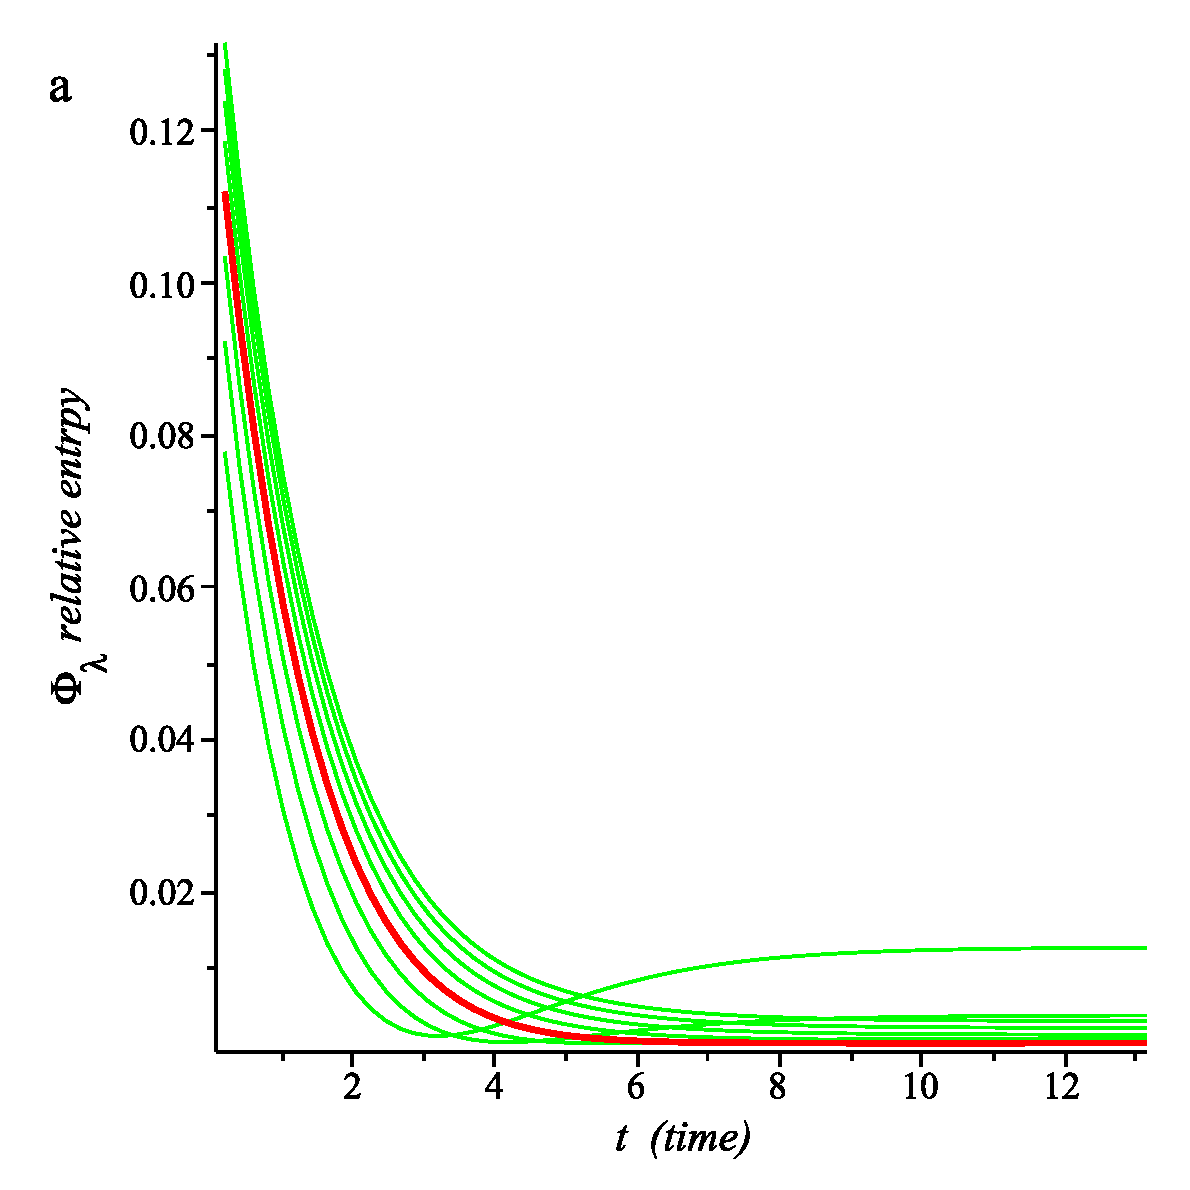
\includegraphics[width=2.5in]{fig_4a.eps}  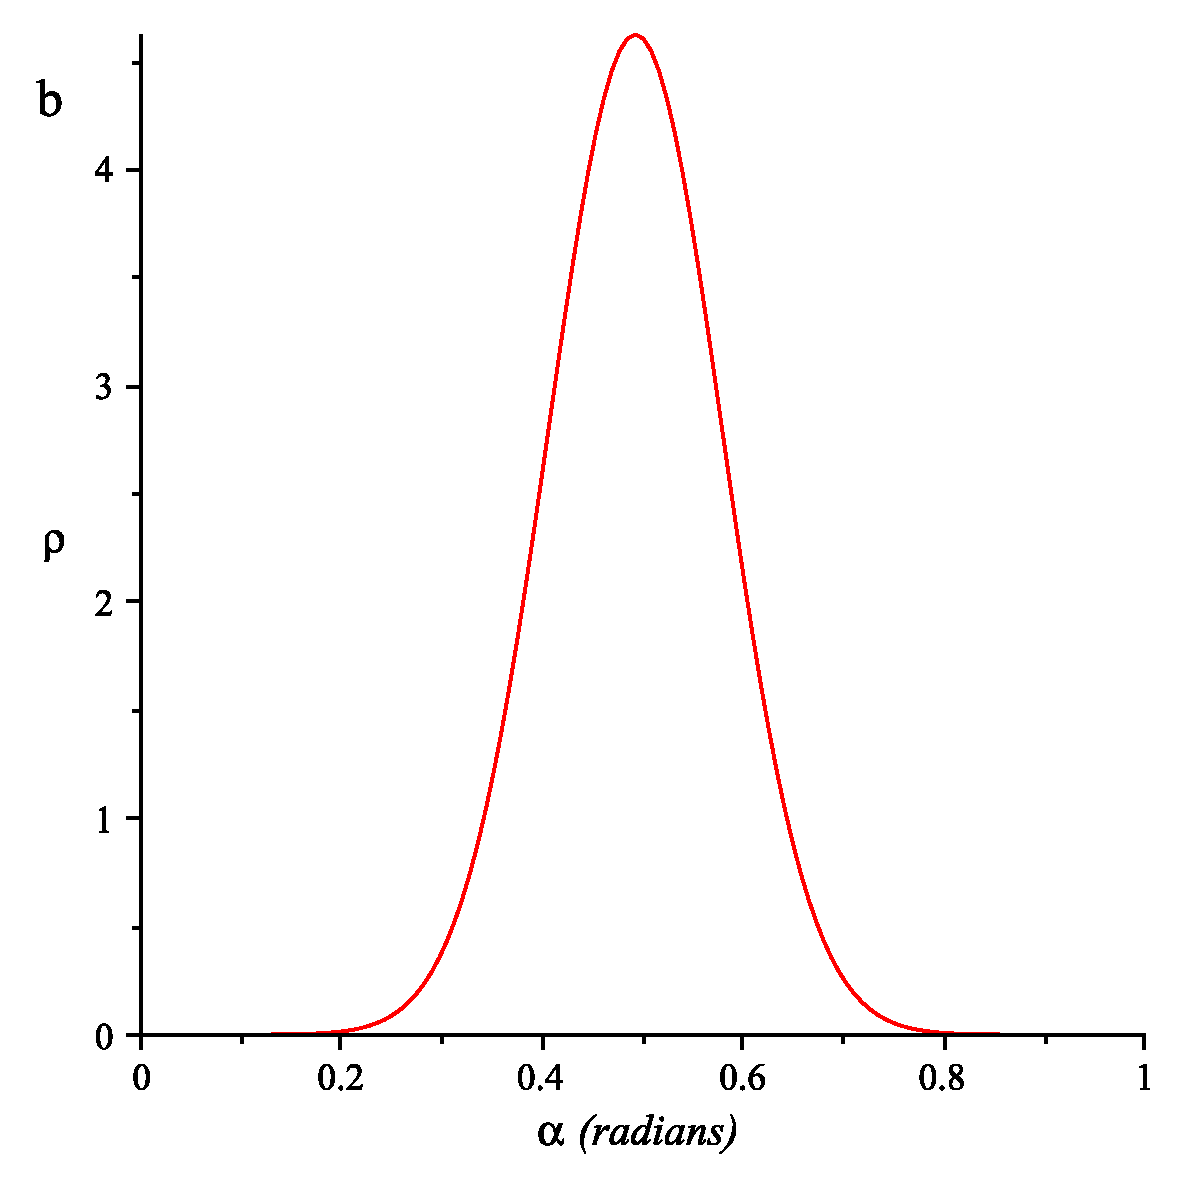
\includegraphics[width=2.5in]{fig_4b.eps}
   \caption{\label{fig:FP} (Color online) (a) The relative entropy $\Phi_\sigma$ of the solution $u(x,t)$ of the Fokker-Planck Equation (\ref{FP}) for the potential  $\psi(x) = 1 + r (x - \frac{1}{2})^2, r = 2,$ with the choice  $\lambda = \sigma = 0.0296915$, computed by a routine numerical method,  compared with a sequence of  $\Phi_\lambda$  with the curve for  $\sigma = 0.0296915$ noted in red.  The values of  $\lambda$  correspond to  $\rho_\lambda$  with  $\max \rho_\sigma/2  \leqq \max \rho_\lambda  \leqq (3/2) \max \rho_\sigma$  (b)  The computed equlibrium solution, which is indistinguishable from  $\rho_\sigma,$  the Boltzmann distribution of  (\ref{relent}).}
\end{figure}

\begin{figure}[htbp] 
   \centering
   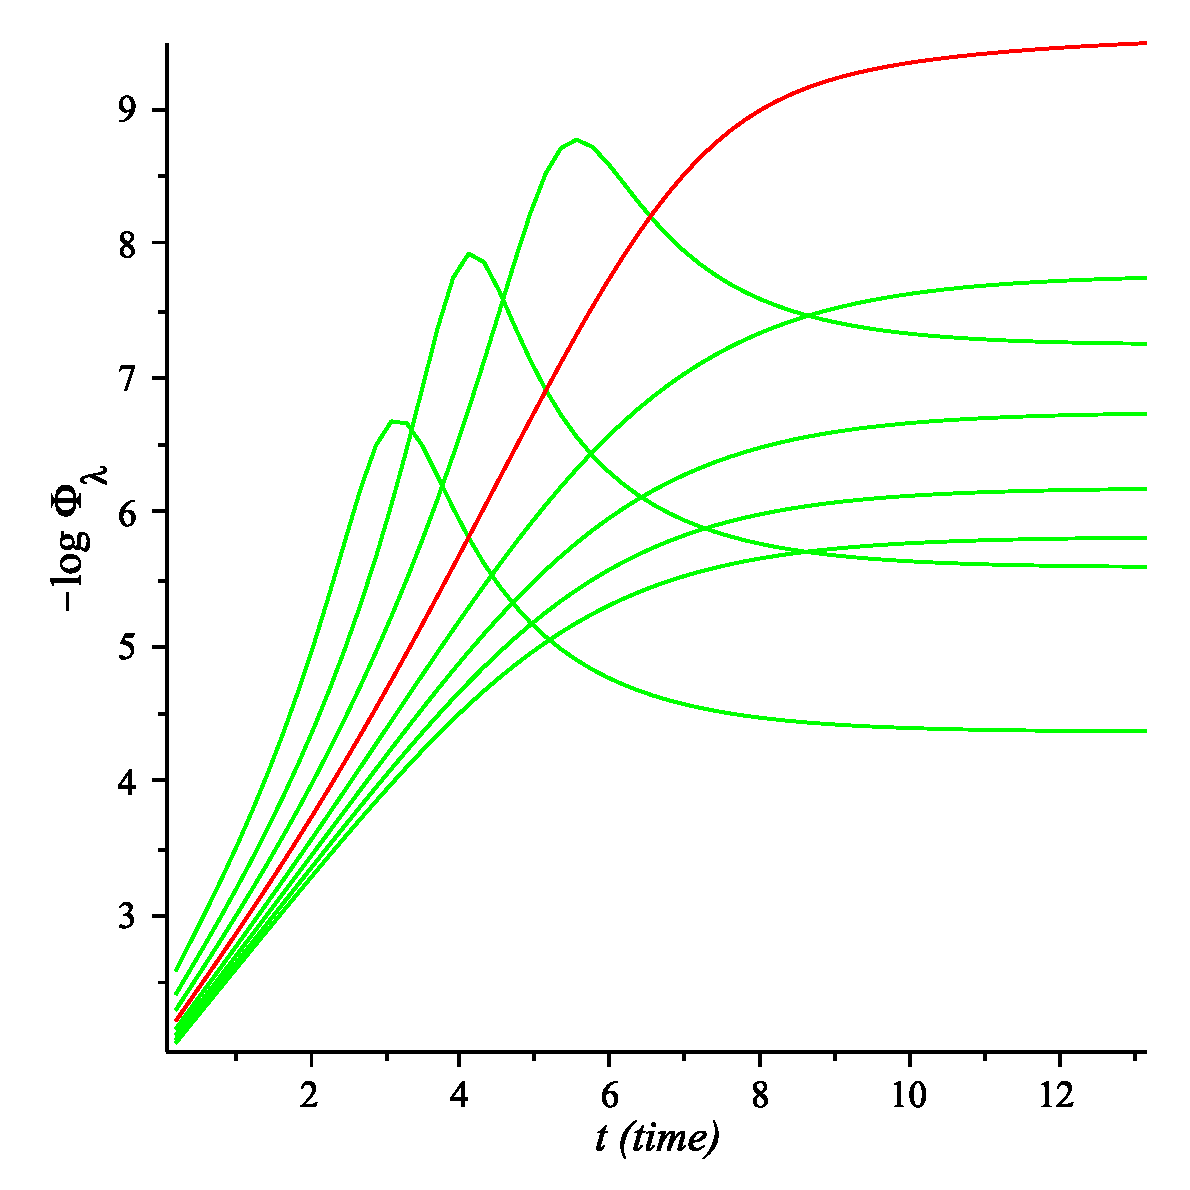
\includegraphics[width=2.5in]{fig_5.eps} 
   \caption{ \label{fig:logPhi}(Color online) Plots of  $-\log \Phi_\lambda $  vs. $t$  with   $-\log \Phi_\sigma $  in red for the solution of  (\ref{FP}), cf. FIG. \ref{fig:FP}.  The plot illustrates that $\Phi_\sigma$  decreases exponentially to  $0$  but that  $\Phi_\lambda$  for choices of  $\lambda \neq \sigma$ do not have this property.}
\end{figure}
Therefore, we seek to identify the particular  $\lambda = \sigma$  for which  $\Phi_\sigma$ defined by the GBCD statistic  $\rho$  tends monotonely to the minimum of all the $\{ \Phi_\lambda \}$  as  $t$  becomes large.  The empirical GBCD  $\rho$  is a statistic and so the minimum of all the  $\{ \Phi_\lambda \}$  may not be zero.  So we must proceed to ask if the terminal, or equilibrium, empirical distribution  $\rho$  is equal, that is, reasonably close, to  $\rho_\sigma$ given by the formula (\ref{bol}).  This is the essence of our validation procedure.  For our purposes, we simply decide the question of equality by inspection.  

With validation we would gain qualitative properties of solutions of  (\ref{FP}):  If we find the correct choice for  $\lambda = \sigma$, then from our discussion above,
\begin{itemize}
\item $\rho(\alpha,t) \rightarrow \rho_\sigma(\alpha)$ as $t \rightarrow \infty$, and
\item this convergence is exponentially fast,
\end{itemize} 
and otherwise these properties fail.

In this context, determining a parameter on the basis of its thermodynamic restrictions is well known.  A novelty here is its use in a nonequilibrium setting, cf. also  \cite{ISI:000270383400046,ISI:000270383400047,ISI:000270383400048}.


To understand our implementation, we offer an illustration using the solution of the (\ref{FP})  itself,  $u$  computed on  $\Omega = (0,1)$  with the choices  $\psi(x) = 1 + r(x-1/2)^2, r = 2,$  and  $\lambda = \sigma = 0.0296915$,  and a collection of relative entropy plots $\{ \Phi_\lambda \}$  where values of  $\lambda$  are close to  $\sigma$, cf. FIG.~\ref{fig:FP}(a).  The plot of  $\Phi_\sigma$ vs. time $t$  is noted in red and  it is decreasing and tends to  $0$.  A glance at the resulting equilibrium  $u$, FIG.~\ref{fig:FP}(b),  identifies it as the Boltzmann distribution  $\rho_\sigma$, as constructed.  In Fig \ref{fig:logPhi}, plots of  $-\log \Phi_\lambda$  are shown, illustrating that   $-\log \Phi_\sigma$  increases linearly, or   $\Phi_\sigma$  decreases exponentially while  $\Phi_\lambda$  for  $\lambda \neq \sigma$  does not have this property.


For the simplified coarsening model, we consider
\begin{equation} \label{OUpot}
\psi(\alpha) = 1 + 2 \alpha^2, \ \alpha \in \Omega = (-\frac{\pi}{4},\frac{\pi}{4}),
\end{equation}
and shall identify a unique such parameter, which we label  $\sigma,$  by seeking the minimum of the relative entropy (\ref{relent})  and then comparing it with  $\rho_\sigma$.  This   $\psi$  is the development to second order of   $\psi(\alpha) = 1 + 0.5 \sin^22\alpha$  used in the 2D simulation.  Moreover, since the potential is quadratic, it represents a version of the Ornstein-Uhlenbeck process\cite{DK:vankampen}, what we computed above directly.  To proceed, we must agree upon which time  $T_\infty$  represents time equals infinity.  For the simplified critical event model we are considering, it is clear that by computing for a sufficiently long time all cells will be gone.  This time may be quite long.  We choose the time parameter so that  $80 \%$  of segments have been deleted, which corresponds to the stationary configuration in the two-dimensional simulation.  For the simplifed model simulation, this time is   $T_\infty=T(80\%) =$ 6.73.  For comparison, $T(90\%) = $ 30  and  $T(95\%) =$103.  There may be additional criteria for choosing a terminal time  $T_\infty$  in the neighborhood of  $T(80\%)$  and we may wish to discuss this later.

This simulation is initialized with  $2^{15}+1$ cells and approximately  155  trial distributions $\rho_j$  are collected at 200 rearrangement event intervals.  155 trial relative entropies are constructed from gaussians $\rho_{\lambda_j}$  satisfying
\begin{equation} \label{gauss_selection}   \rho_{\lambda_j}(0) =  \max \rho_{\lambda_j }= \max \rho_j. \end{equation}
Some of these are shown in FIG.~\ref{fig:OUsimp}(a).  The empirical  GBCD  is compared with the appropriate Boltzmann distribution in FIG.~\ref{fig:OUsimp}(b).
\begin{figure}[htbp] 
   \centering
   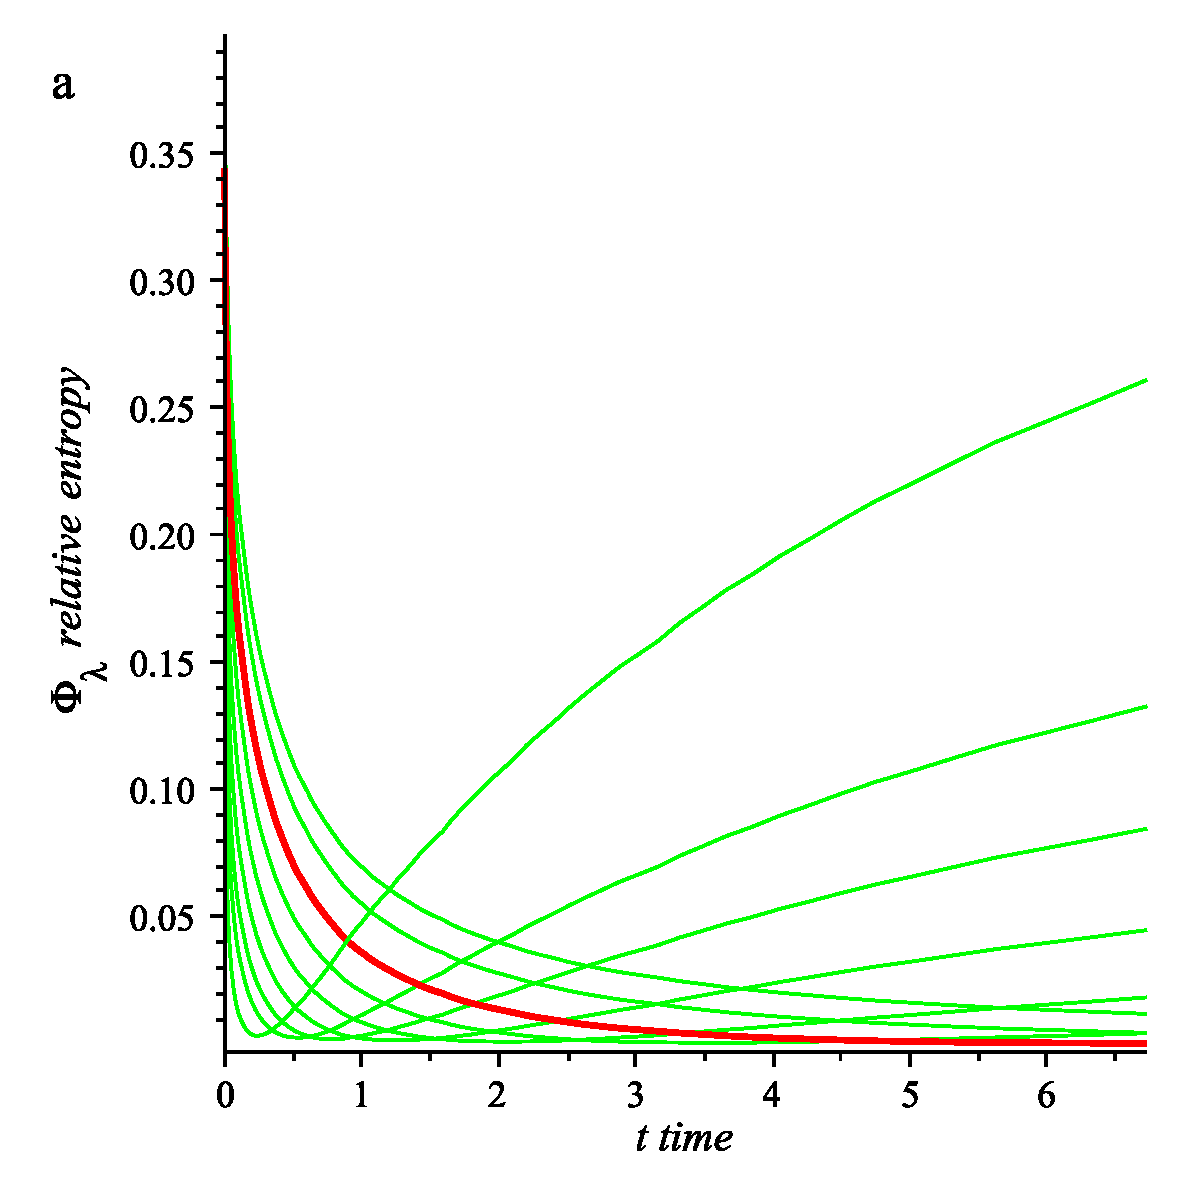
\includegraphics[width=2.5in]{fig_6a.eps}  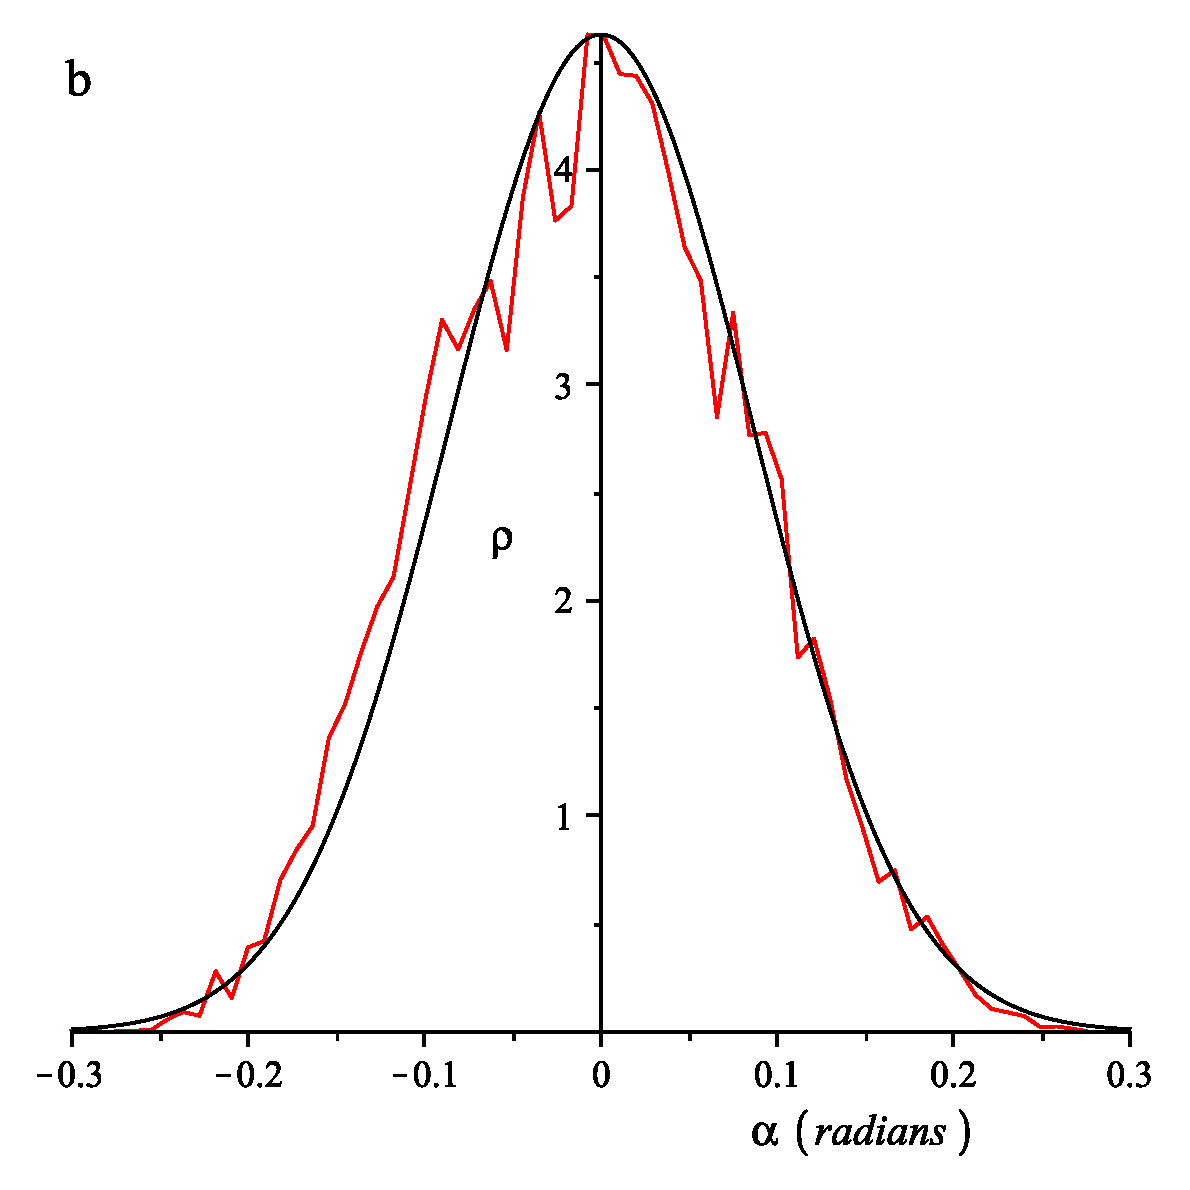
\includegraphics[width=2.5in]{fig_6b.eps} 
   \caption{ \label{fig:OUsimp} (Color online) Graphical results for the simplified coarsening model with potential  (\ref{OUpot}).  (a) Relative entropy plots for values of  $\lambda$  chosen according to (\ref{gauss_selection}) with  $\Phi_\sigma$ noted in red.  The value of  $\sigma =  0.0296915$.  (b)  Empirical GBCD at time  $T = T_\infty$ in red compared with  $\rho_\sigma$ in black.}
\end{figure}

We include the plots of  $-\log \Phi_\lambda$, FIG.\ref{fig:PRB_OU_logrelent},  which suggests that  $\Phi_\sigma$  decays exponentially to its minimum whereas a  $\Phi_\lambda$  corresponding to a other values of  $\lambda$  do not.
\begin{figure}[htbp] 
   \centering
   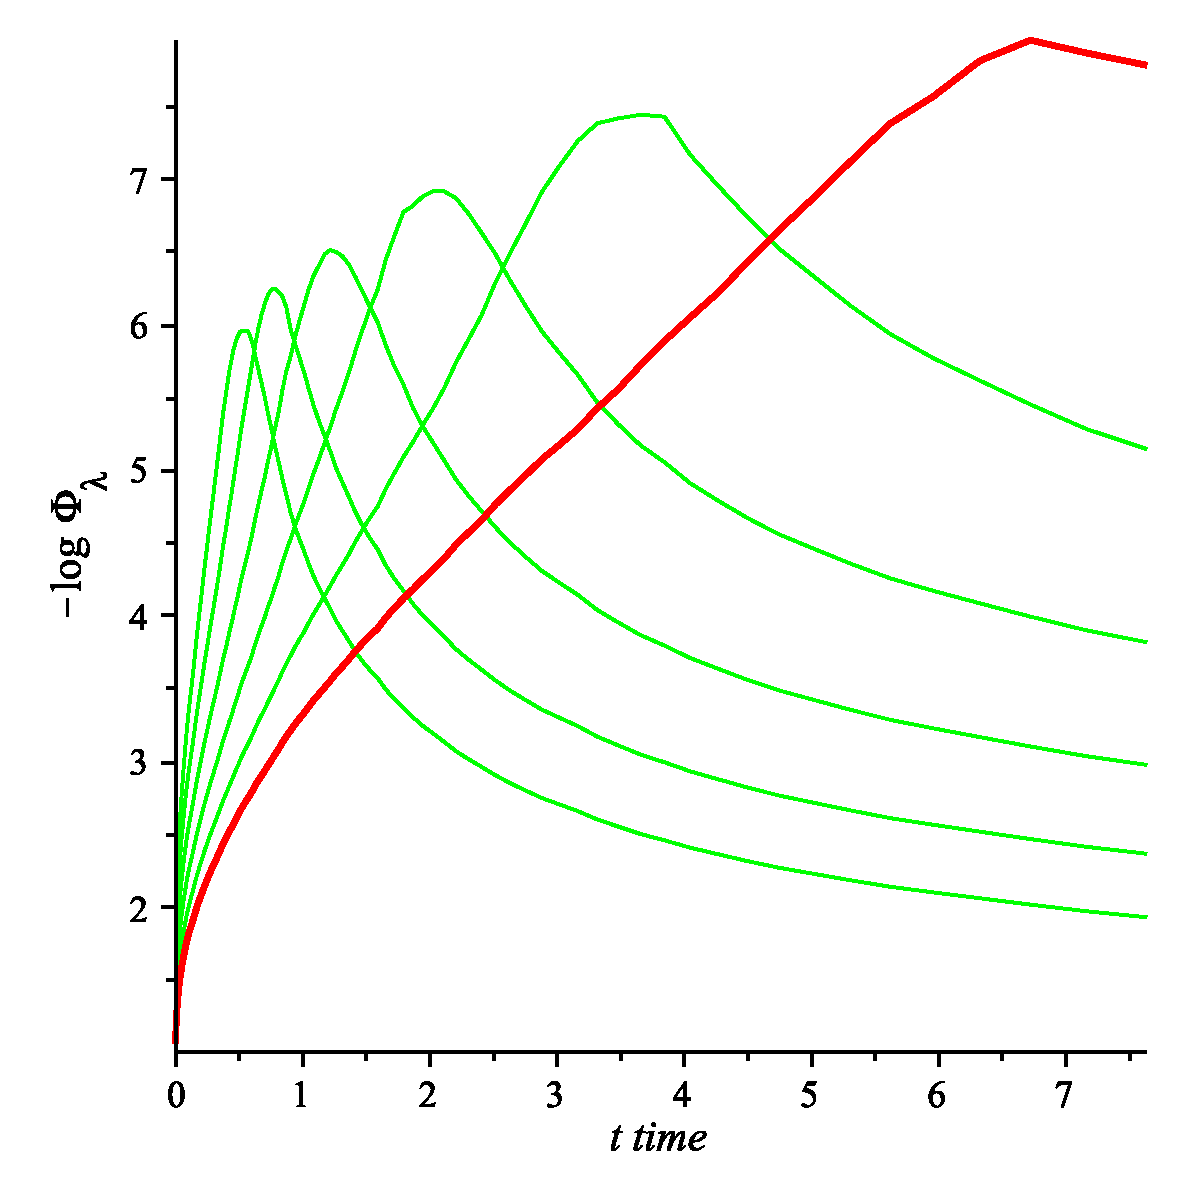
\includegraphics[width=2.5in]{fig_7.eps} 
   \caption{\label{fig:PRB_OU_logrelent} (Color online) Plots of  $ -\log \Phi_\lambda $  vs. $t$  with   $-\log \Phi_\sigma, \sigma =  0.0296915$,  in red for the simplified coarsening model with potential  (\ref{OUpot}).  It shows that
    $\Phi_\sigma$  decays exponentially to its minimum at time $T_\infty$.}
\end{figure}

For a second example to illustrate the method, we consider the potential
\begin{equation} \label{4pot}
\psi(\alpha) = 1 + \epsilon \alpha^4, \ \alpha \in \Omega, \ \epsilon = 8.
\end{equation}
This choice,  $\epsilon = 8,$  corresponds to the first order terms in the two dimensional quartic energy density we discuss in the next section.  Also here in FIG.~\ref{fig:OU4} one sees very good agreement between the empirical GBCD and the appropriate Boltzmann distribution.
\begin{figure}[htbp] 
   \centering
   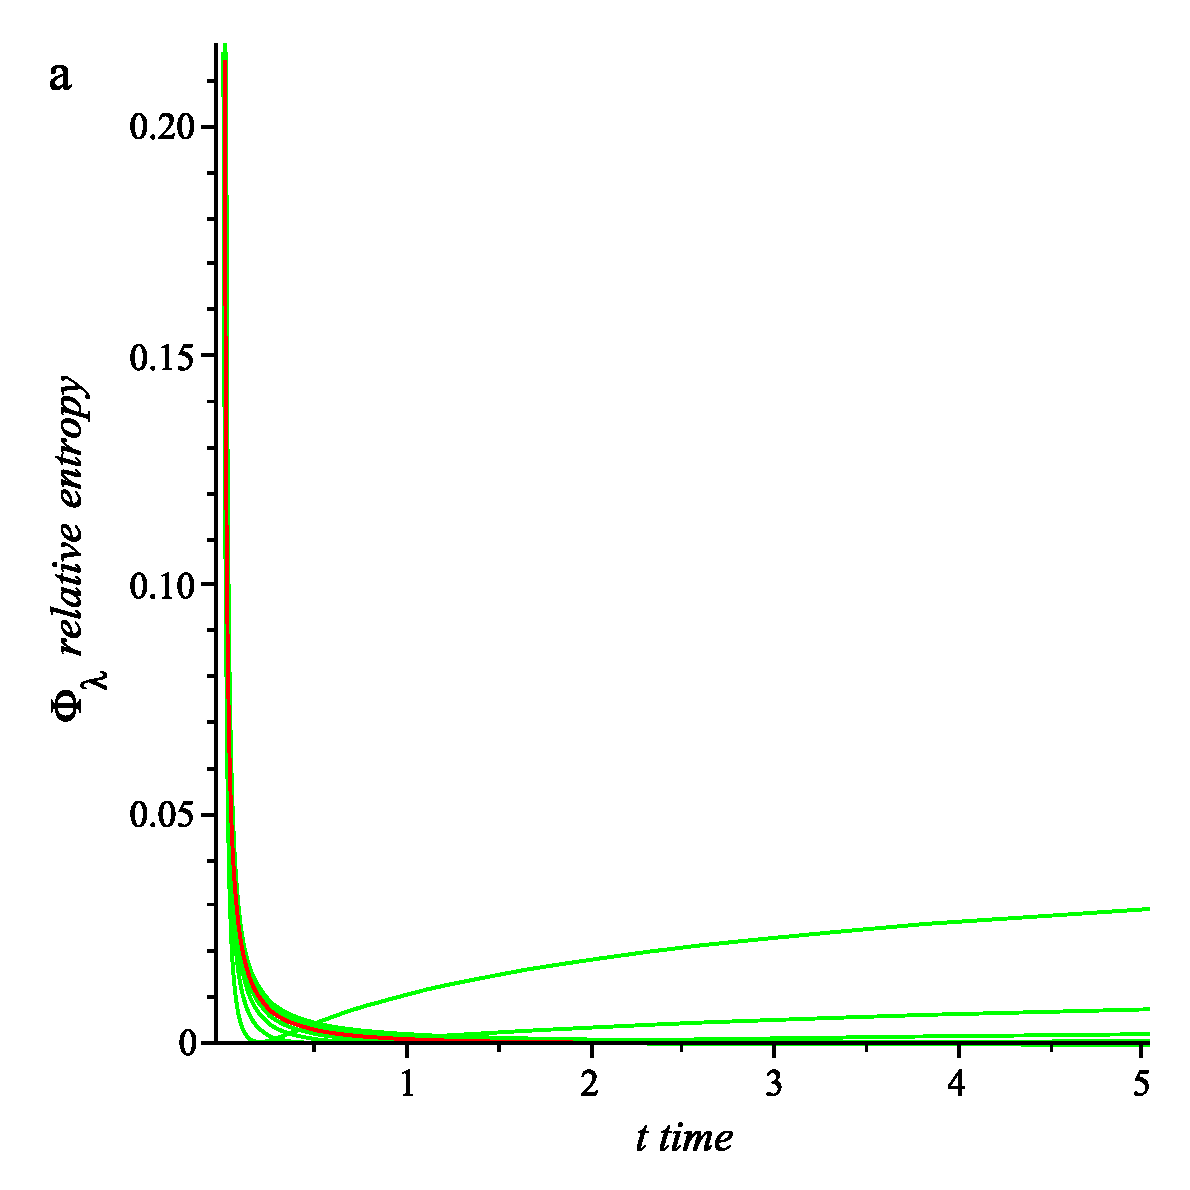
\includegraphics[width=2.5in]{fig_8a.eps}  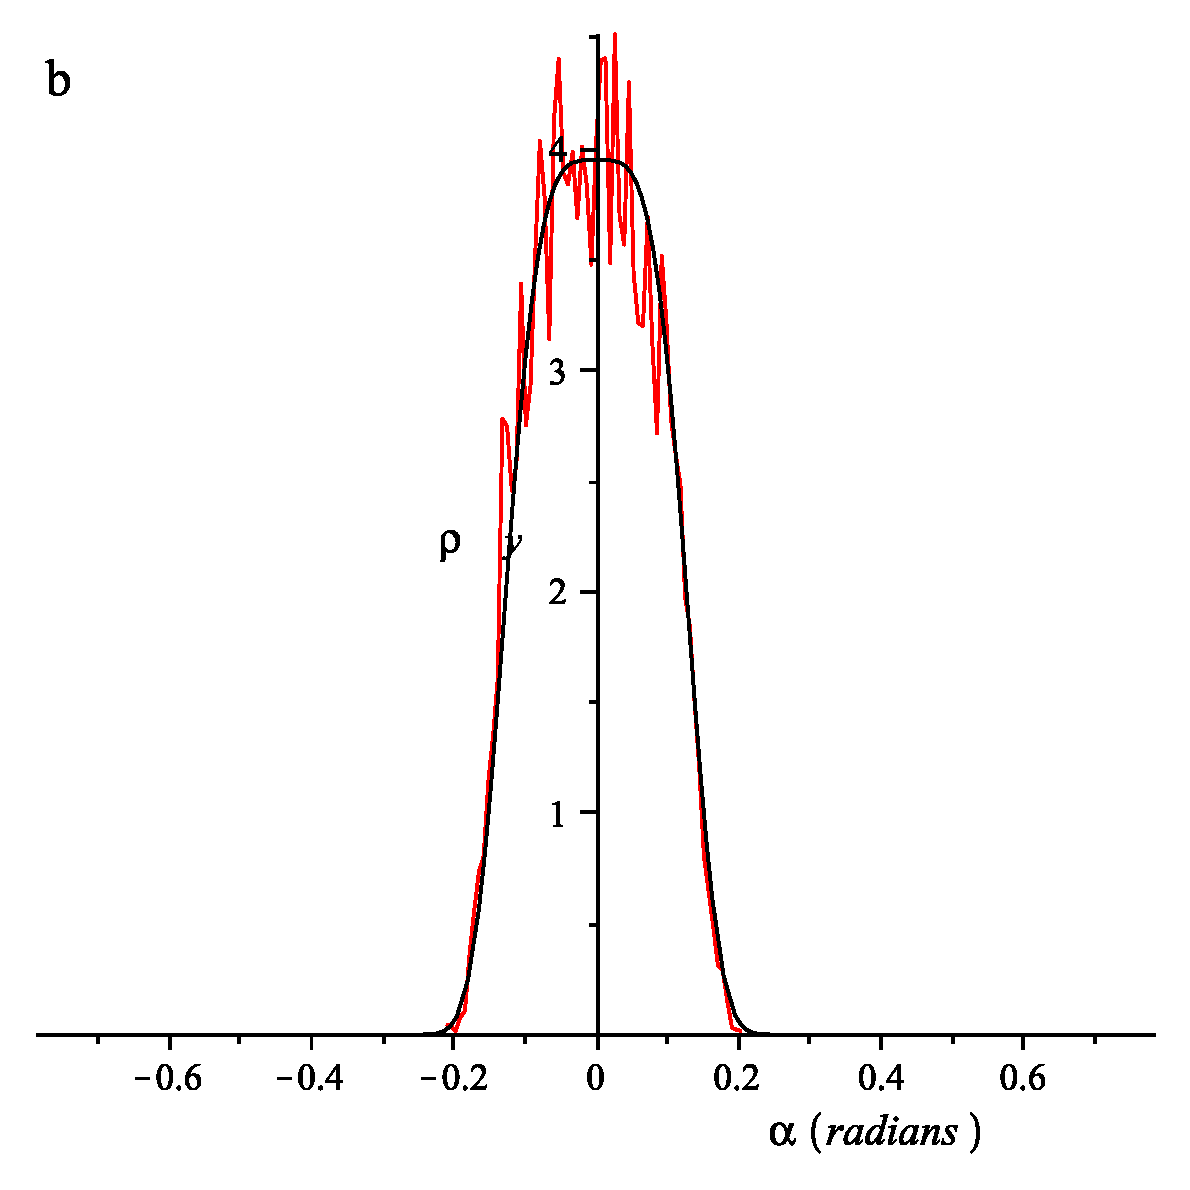
\includegraphics[width=2.5in]{fig_8b.eps}
   \caption{ \label{fig:OU4} (Color online) Graphical results for the simplfied coarsening model with potential  (\ref{4pot}).  (a) Relative entropy plot for selected values of  $\lambda$  with  $\Phi_\sigma$ noted in red.  The value of  $\sigma=   0.003033356683$  and is ascertained at the time  $T = T_\infty$  corresponding to  $80\%$ of cells deleted.  (b)  Empirical GBCD at time  $T = T_\infty$ in red compared with  $\rho_\sigma$  in black. }
\end{figure}



\section{The entropy method for the GBCD}  We shall apply the method of Section \ref{validation} to the GBCD harvested from the 2D simulation.  We consider first a typical simulation with the energy density  
\begin{equation} \label{quadratic}
\psi(\alpha) = 1 + \epsilon (\sin 2\alpha)^2,  \ -\frac{\pi}{4} \leqq \alpha \leqq \frac{\pi}{4}, \ \epsilon = 1/2,
\end{equation} FIG.~\ref{fig:psi},   initialized with  $10^4$  cells and normally distributed misorientation angles and terminated when 2000 cells remain.  At this stage, the simulation is essentially stagnant.  Possible parameters  $\lambda$  are constructed similarly to those of the simplified coarsening model:  From the maximum of a harvested GBCD, we construct the gaussian with the same maximum.  This determines a value of  $\lambda$  which is used to define  $\rho_\lambda$  in  (\ref{bol})  for the density  \ref{quadratic}.  This  $\rho_\lambda$ then  defines a trial relative entropy via (\ref{relent}). 
\begin{figure}[htbp] 
   \centering
   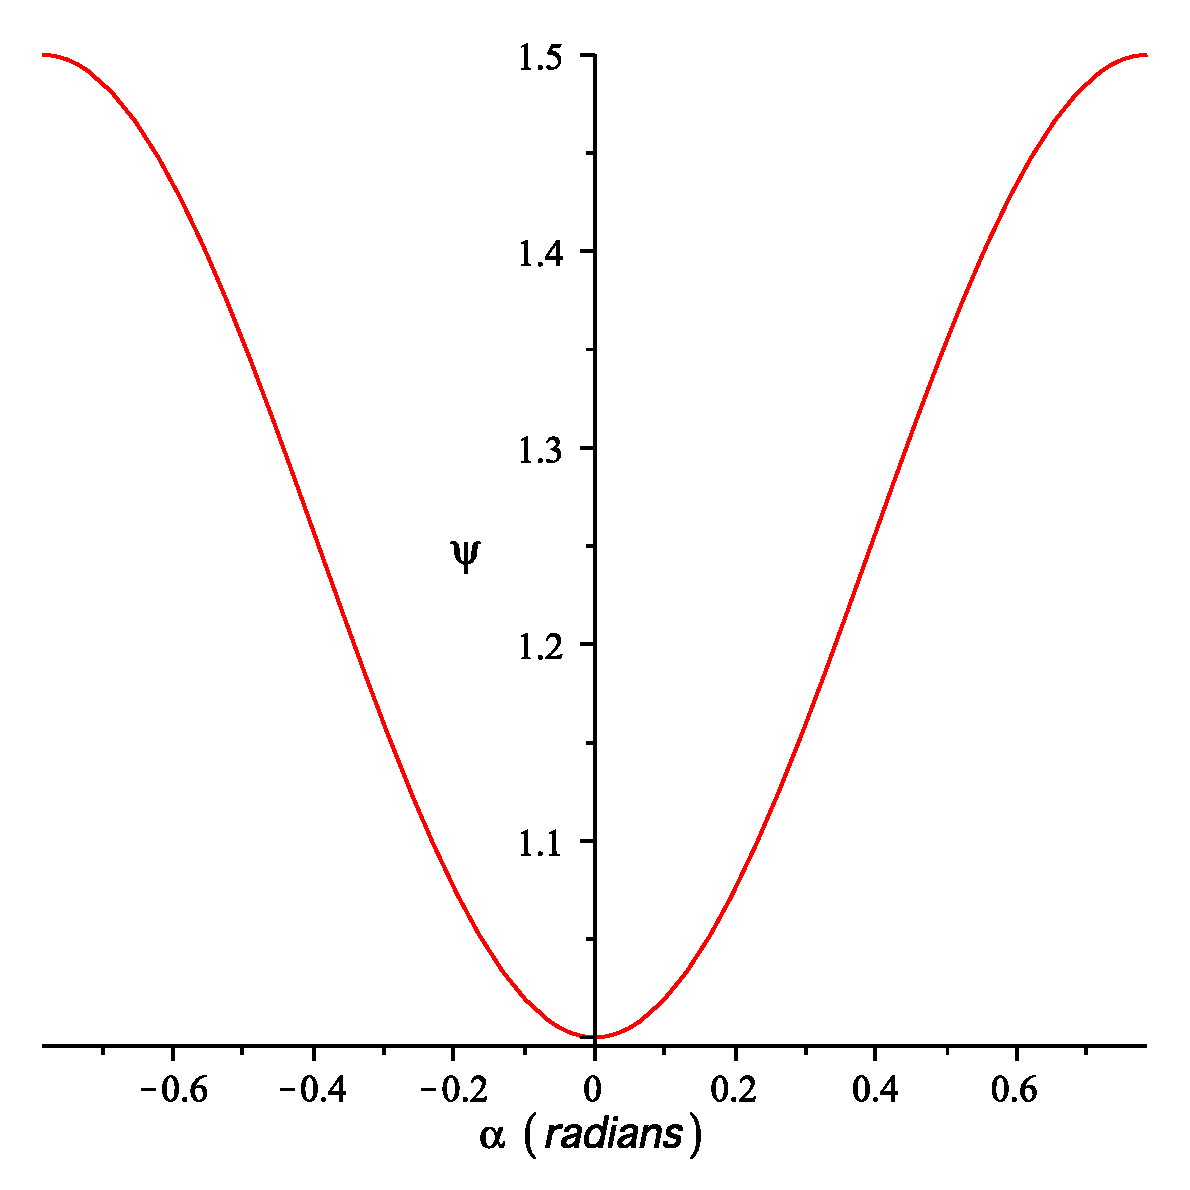
\includegraphics[width=2.5in]{fig_9.eps} 
   \caption{\label{fig:psi} (Color online) The energy density  $\psi(\alpha) = 1 + \epsilon \sin^22\alpha, \ |\alpha| < \pi/4, \ \epsilon = \frac{1}{2}.$ }
\end{figure}

\begin{figure}[h]
   \centering
   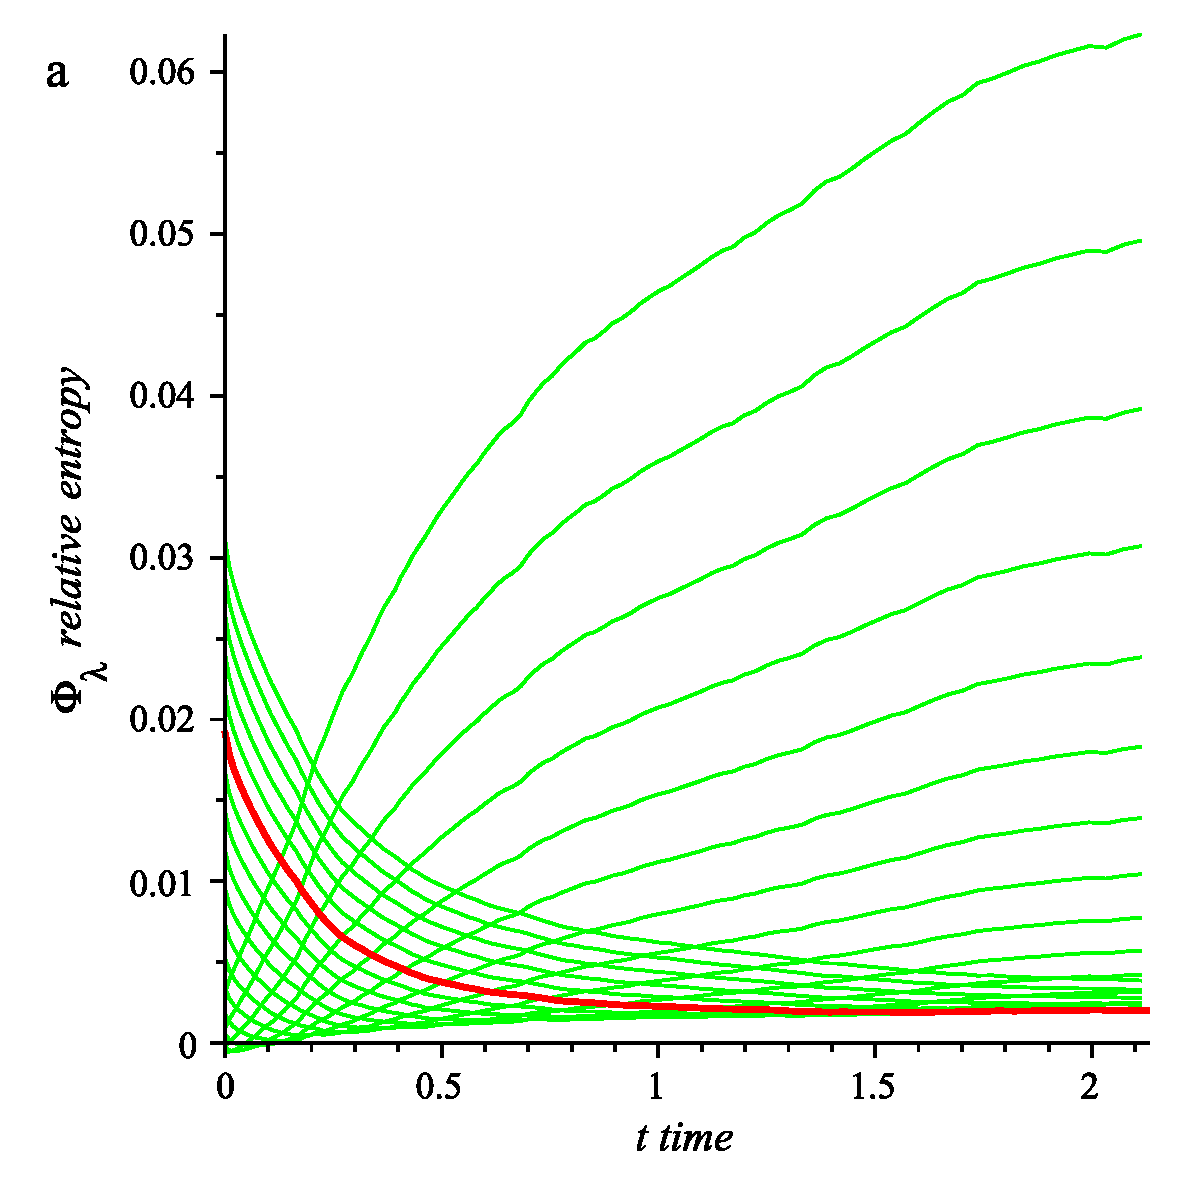
\includegraphics[width=2.5in]{fig_10a.eps}  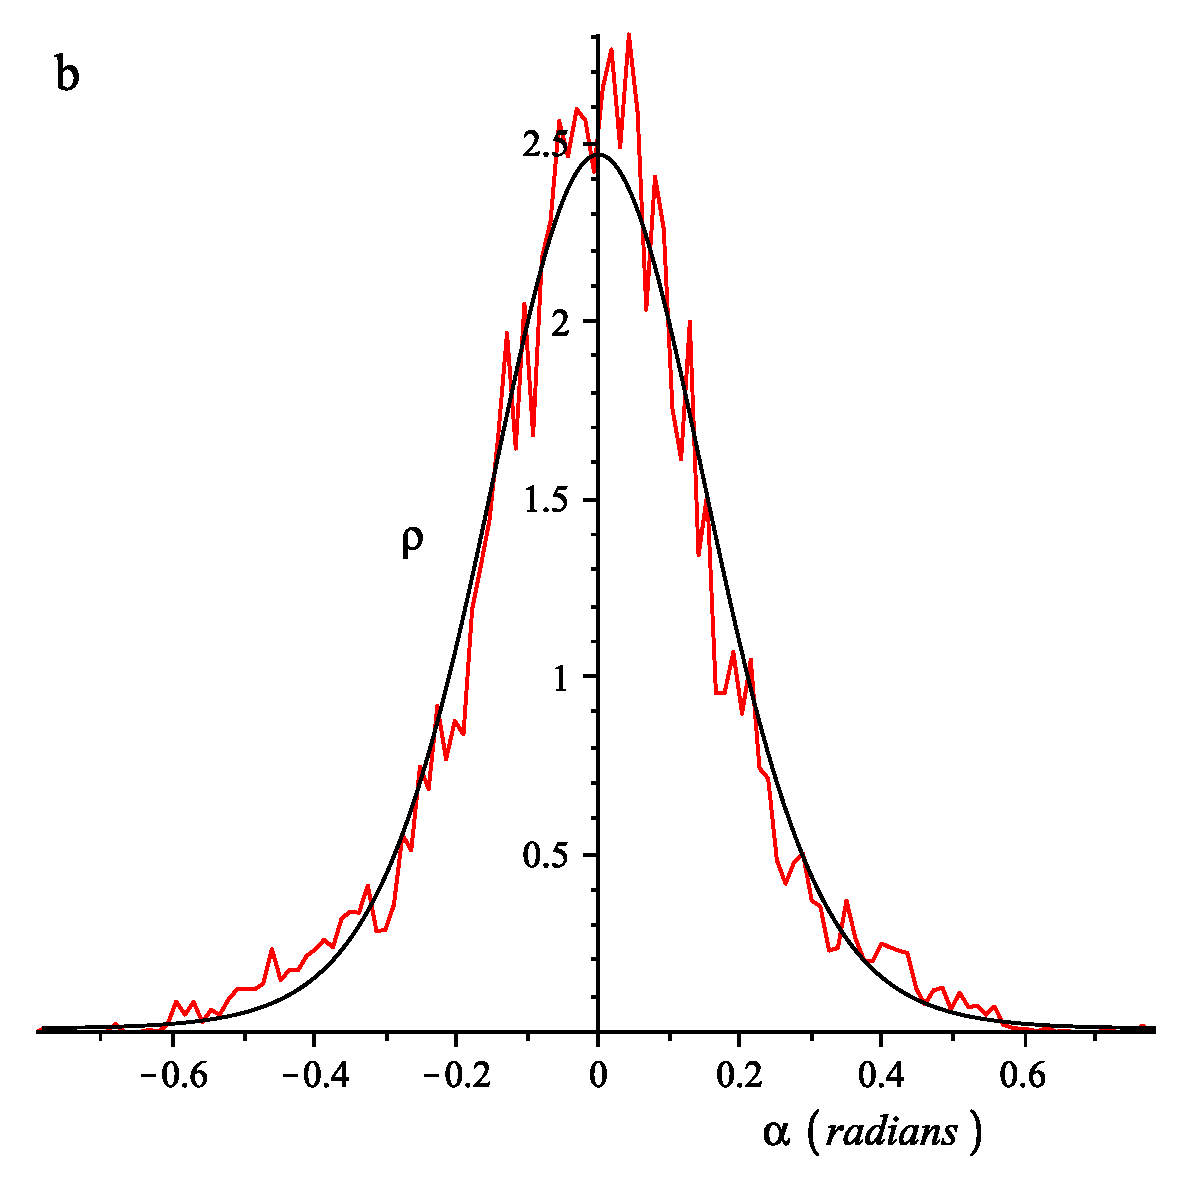
\includegraphics[width=2.5in]{fig_10b.eps}
   \caption{  \label{fig:success} (Color online) (a) The relative entropy of the grain growth simulation with energy density  (\ref{quadratic}) for a sequence of  $\Phi_\lambda$  vs. $t$ with the optimal choice  $\sigma \approx 0.1$ noted in red.  (b)  Comparison of the empirical GBCD distribution at time  $t=2$, when  $80\%$  of the cells have been deleted, with  $\rho_\sigma,$  the Boltzmann distribution of  (\ref{bol}).}  
   \end{figure}

We now identify the parameter  $\sigma$  which turns out to be  $\sigma \approx 0.1$, FIG.~\ref{fig:success}(a).  In  FIG.~\ref{fig:success}(b) the empirical GBCD is compared with the Boltzmann distribution with parameter determined by FIG.~\ref{fig:success}(a), showing excellent agreement.  From FIG.~\ref{fig:success_log}, we see that this relative entropy  $\Phi_\sigma$  has exponential decay until it reaches a value of about  1.5, when it remains constant.  The solution itself thus tends exponentially (in  $L^1$) to its limit  $\rho_\sigma$  by the Csiszar-Kullback Inequality.  

FIG.~\ref{fig:5success} shows that averaging over a few trials, five in this case, the empirical GBCD's approach the Boltzmann distributiion $\rho_\sigma$ of  (\ref{bol})  quite closely.
\begin{figure}[htbp] 
   \centering
   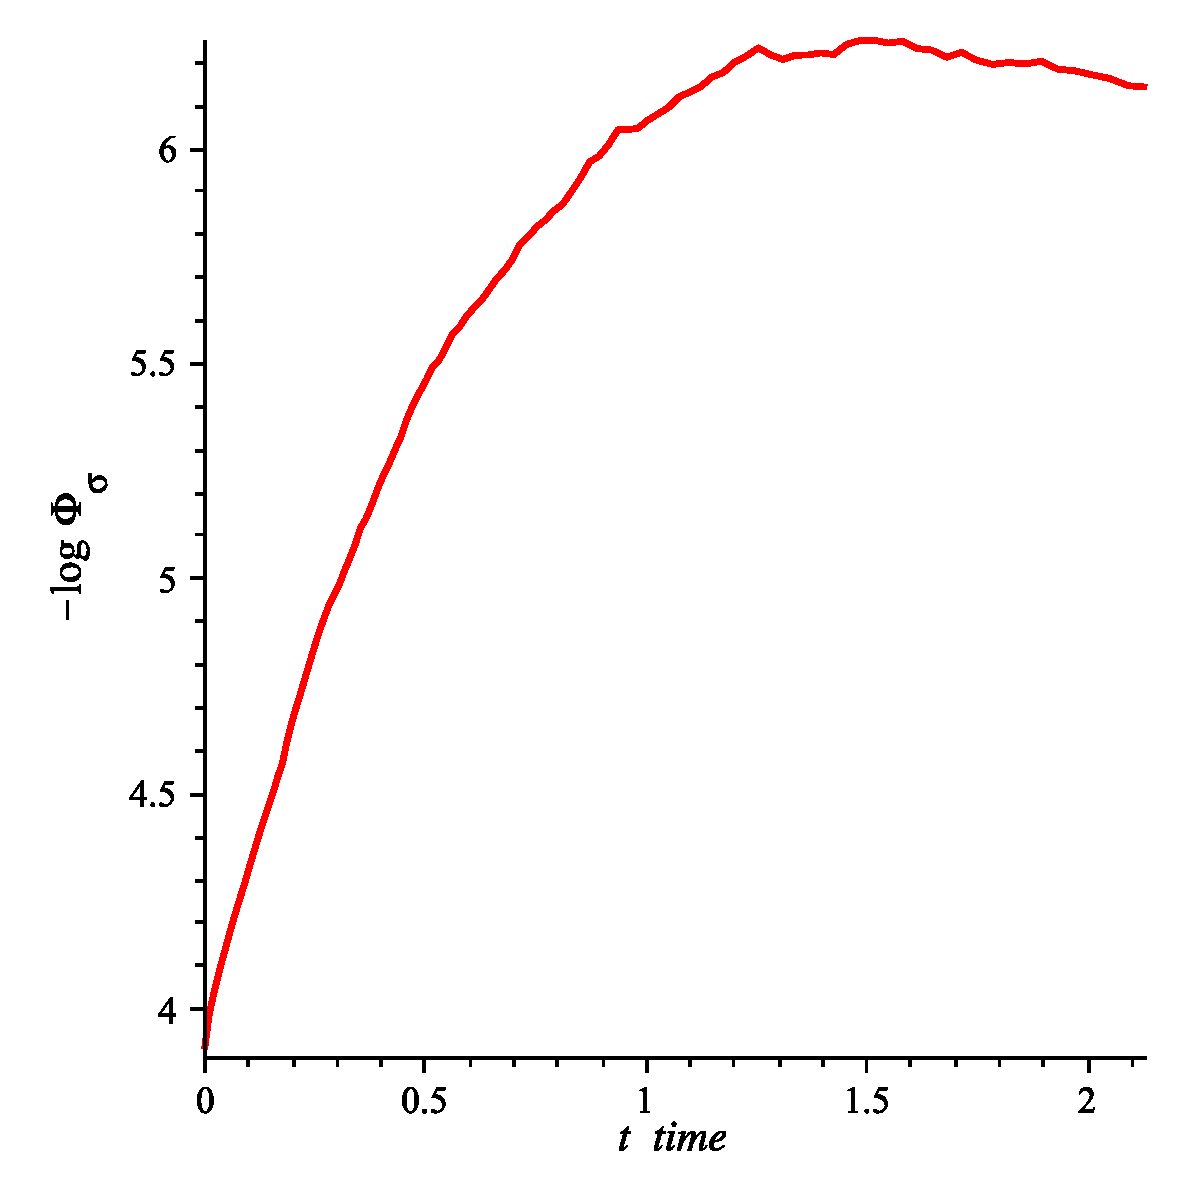
\includegraphics[width=2.5in]{fig_11.eps} 
   \caption{ \label{fig:success_log} (Color online) Plot of  $-\log \Phi_\sigma$ vs. $t$  with energy density  (\ref{quadratic}).  It is approximately linear until it becomes constant showing that  $\Phi_\sigma$  decays exponentially}
\end{figure}
\begin{figure}[htbp] 
   \centering
   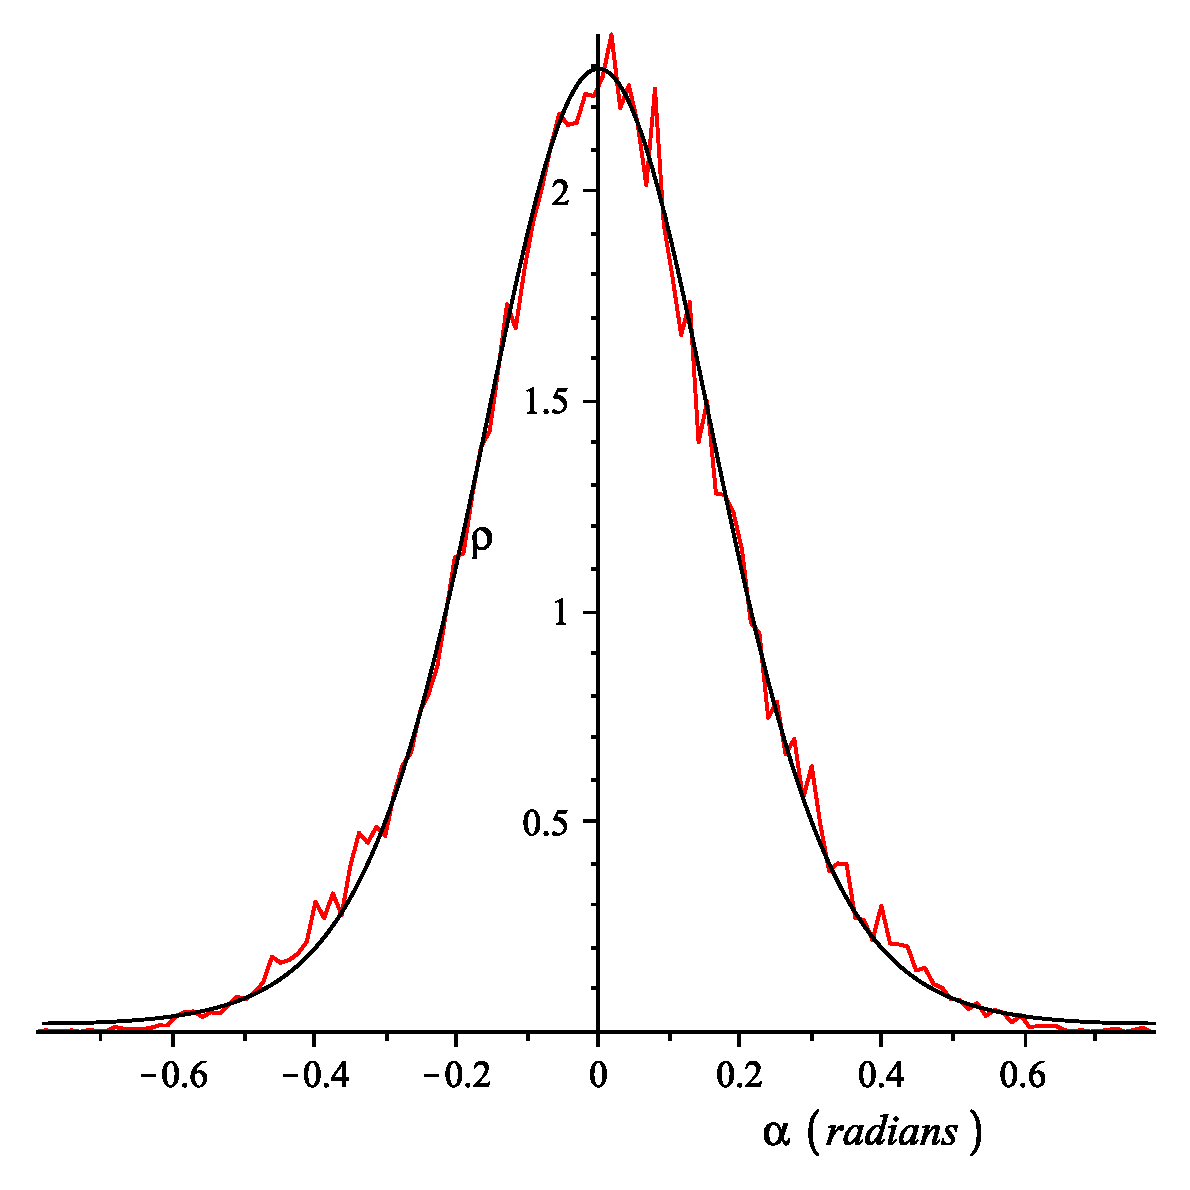
\includegraphics[width = 2.5in]{fig_12.eps}
   \caption{ \label{fig:5success} (Color online) GBCD (red) and Boltzmann distribution (black) for the potential  $\psi$  of (\ref{quadratic})  with parameter $\sigma \approx 0.1$  as predicted by our theory.  This GBCD is averaged over 5 trials.}
\end{figure}
A second example presented here is a quartic energy  
\begin{equation} \label{quartic}
\psi(\alpha) = 1 + \epsilon(\sin 2\alpha)^4, \ -\frac{\pi}{4} \leqq \alpha \leqq \frac{\pi}{4}, \ \epsilon = 1/2.
\end{equation}  Again, a configuration of  $10^4$ cells is initialized with normally distributed misorientations and, this time, the computation proceeds until about $1000$ cells remain.  The relative entropy and the equilibrium Boltzmann statistic stabilize when $2000$ cells remain.  
\begin{figure}[h] 
   \centering
   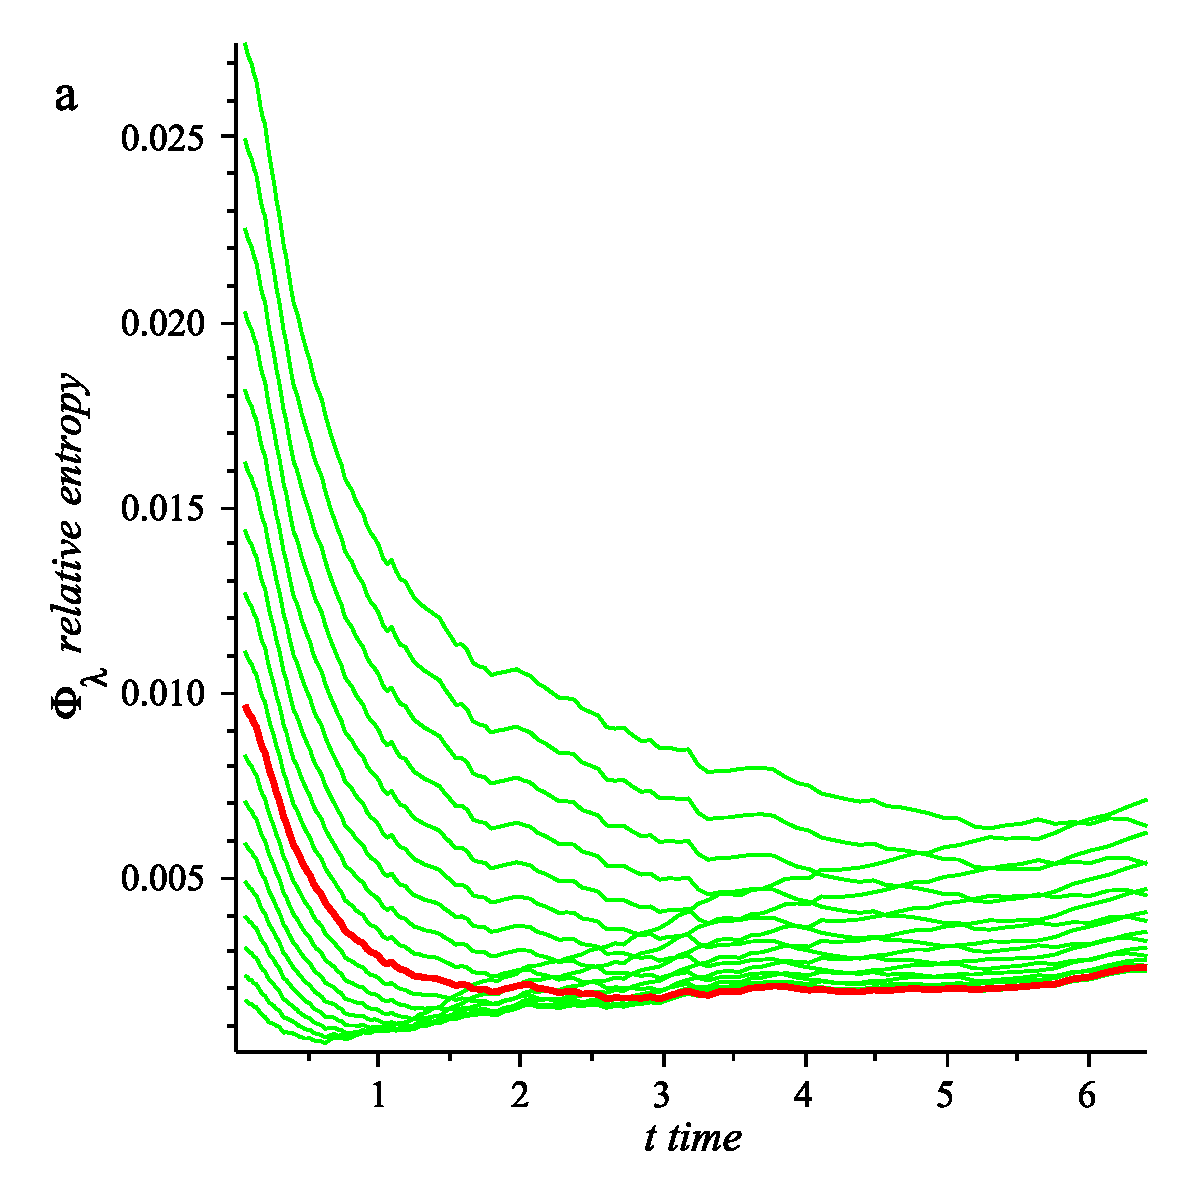
\includegraphics[width=2.5in]{fig_13a.eps}  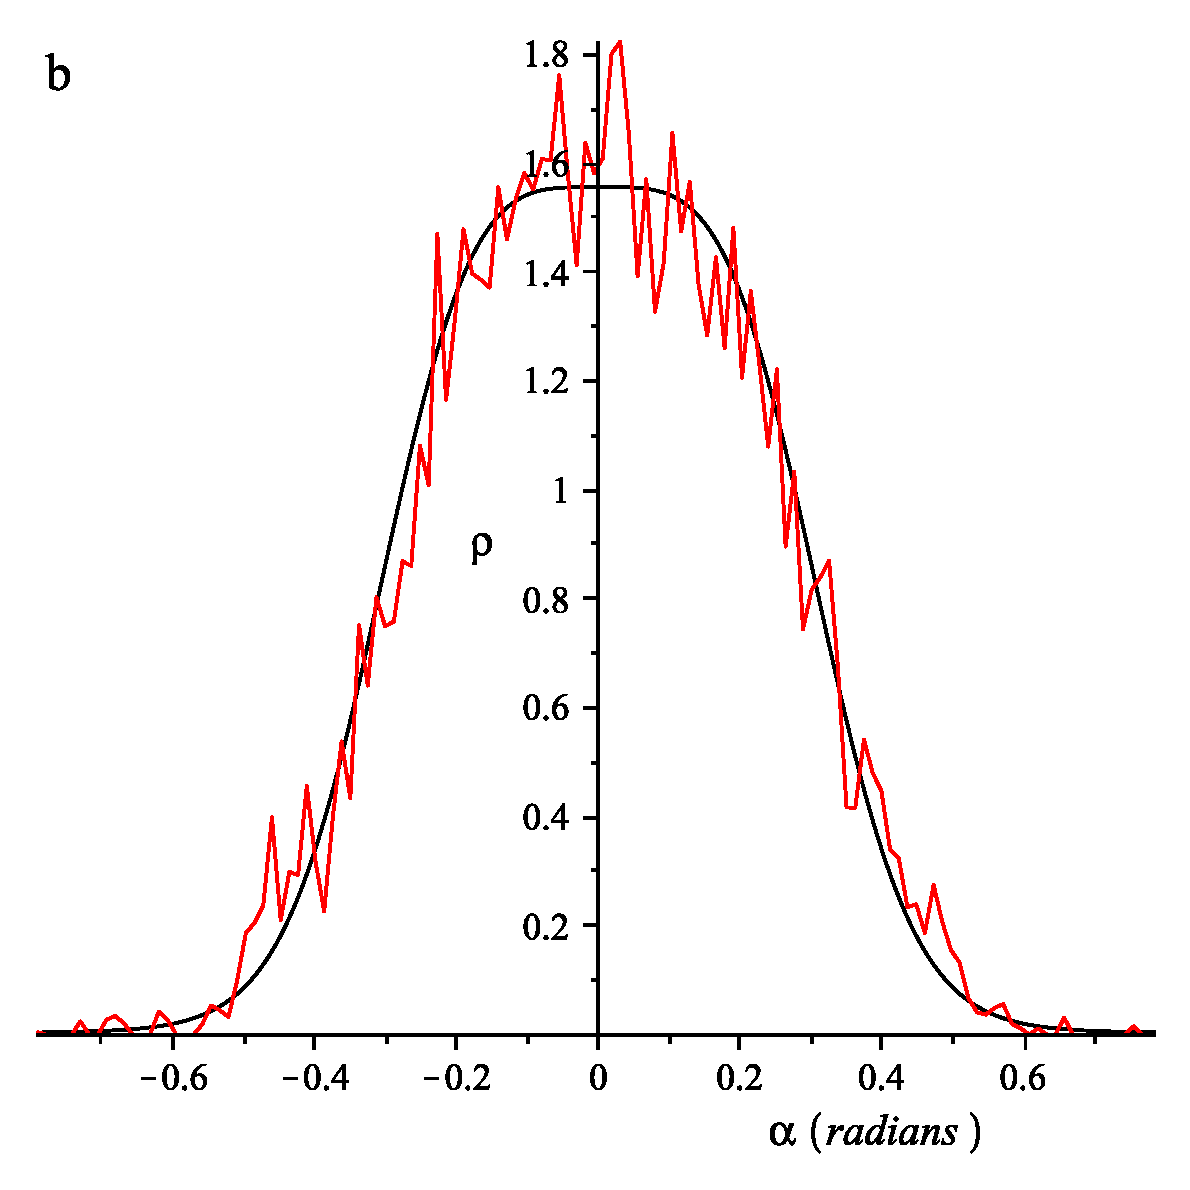
\includegraphics[width=2.5in]{fig_13b.eps}
   \caption{   \label{fig:success4} (Color online) (a) The relative entropy of the grain growth simulation with density (\ref{quartic}) for a sequence of  $\Phi_\lambda$  vs. $t$ with the optimal choice  $\sigma \approx 0.08$ noted in red.  (b)  Comparison of the empirical GBCD at time  $t=2$, when  $80\%$  of the cells have been deleted, with  $\rho_\sigma,$  the Boltzmann distribution of  (\ref{bol}).}  
   \end{figure}

With the equilibrium solution in hand, as depicted in FIG~\ref{fig:success4}, we again initialized a configuration of  $10^4$ cells with, on this occasion, misorientations normally distributed in the much narrower range defined by the sides of the solution GBCD.  Since these misorientations see, essentially, only the near minimum of the potential, we would expect the new stationary distribution to be gaussian or random.  However we obtain the same relative entropy curve and equilibrium depicted in FIG.~\ref{fig:success4}.  Although coarsening is not like a molecular system with eternal collisions causing the entire system to equilibrate, the fluctuations of misorientations caused by the `perpetual'  critical events provide the system with a sufficiently ample library to be driven by the given grain boundary energy density.  On the other hand, we may defeat this attribute, for example, with a Read-Shockley type of energy, which is cusp-like near the origin and rises sharply to a maximum.  Near the origin, we obtain a reasonable distribution, however there are otherwise insufficent orientations to populate a Boltzmann distribution, \cite{dk:rexggIV}.

Future work will address the theory when the interfacial energy density  $\psi = \psi(\theta,\alpha)$  depends on both normal angle and misorientation of the interface.  In this context, we have observed that simply resolving the solution of the Fokker-Planck Equation with quartic potential leads to bimodal intermediate distributions, which are the stationary distributions for quartic interfacial energy distributions. \cite{ISI:000184366100003, ISI:000225119800166}  This suggests that this situation represents the quenched solution of a Fokker Planck Equation and a role for the second eigenfunction of the equation.  Other effects will also be studied.  These can be added to the local evolution law, most simply, varying mobility, and other retarding forces such as  triple junction drag.
\section{Discussion/conclusions}  Here we have outlined an entropy based theory of the GBCD which is an upscaling of cell growth according to the two most basic properties of a coarsening network:  a local evolution law and space filling contraints.  
The theory accomodates the irreversibility conferred by the critical events or topological rearrangements which arise during coarsening. Details are given for a model system where the analytical tools are easily exploited and they are seen to describe well the results of two dimensional simulations.  Our principal conclusion is that these events occur preferentially in a manner that renders the GBCD closely related to the solution of a Fokker Planck Equation whose potential is the given interfacial energy density.  This reasoning exploits the recent characterization of Fokker-Planck kinetics as a gradient flow for the free energy.

We note that the theory states in particular that it is the GBCD that is a consequence of the coarsening process.  The traditional texture distribution is the orientation distribution  (OD), the distribution of grain orientations.  The GBCD is the distribution of differences of the OD, basically the convolution of the OD with itself.  This relationship may be inverted, by elementary Fourier analysis, so, in this simple case, the GBCD determines the OD and not the other way around. Therefore, we may expect, in nature, that it is among the processes that determine the OD.


\section*{Acknowledgements}
{\footnotesize   This research was done while Y. Epshteyn and R. Sharp were a postdoctoral associates at the Center for Nonlinear Analysis.  We are grateful to our colleagues G. Rohrer, A. D. Rollett, R. Schwab, and R. Suter for their collaboration.  Research supported by NSF DMR0520425, DMS 0405343, DMS 0305794, DMS 0806703, DMS 0635983, DMS0915013.}

\begin{thebibliography}{53}%
\makeatletter
\providecommand \@ifxundefined [1]{%
 \@ifx{#1\undefined}
}%
\providecommand \@ifnum [1]{%
 \ifnum #1\expandafter \@firstoftwo
 \else \expandafter \@secondoftwo
 \fi
}%
\providecommand \@ifx [1]{%
 \ifx #1\expandafter \@firstoftwo
 \else \expandafter \@secondoftwo
 \fi
}%
\providecommand \natexlab [1]{#1}%
\providecommand \enquote  [1]{``#1''}%
\providecommand \bibnamefont  [1]{#1}%
\providecommand \bibfnamefont [1]{#1}%
\providecommand \citenamefont [1]{#1}%
\providecommand \href@noop [0]{\@secondoftwo}%
\providecommand \href [0]{\begingroup \@sanitize@url \@href}%
\providecommand \@href[1]{\@@startlink{#1}\@@href}%
\providecommand \@@href[1]{\endgroup#1\@@endlink}%
\providecommand \@sanitize@url [0]{\catcode `\\12\catcode `\$12\catcode
  `\&12\catcode `\#12\catcode `\^12\catcode `\_12\catcode `\%12\relax}%
\providecommand \@@startlink[1]{}%
\providecommand \@@endlink[0]{}%
\providecommand \url  [0]{\begingroup\@sanitize@url \@url }%
\providecommand \@url [1]{\endgroup\@href {#1}{\urlprefix }}%
\providecommand \urlprefix  [0]{URL }%
\providecommand \Eprint [0]{\href }%
\@ifxundefined \urlstyle {%
  \providecommand \doi  [0]{\begingroup \@sanitize@url \@doi}%
  \providecommand \@doi [1]{\endgroup \@@startlink {\doibase
  #1}doi:\discretionary {}{}{}#1\@@endlink }%
}{%
  \providecommand \doi  [0]{doi:\discretionary{}{}{}\begingroup
  \urlstyle{rm}\Url }%
}%
\providecommand \doibase [0]{http://dx.doi.org/}%
\providecommand \Doi [0]{\begingroup \@sanitize@url \@Doi }%
\providecommand \@Doi  [1]{\endgroup\@@startlink{\doibase#1}\@@Doi}%
\providecommand \@@Doi [1]{#1\@@endlink}%
\providecommand \selectlanguage [0]{\@gobble}%
\providecommand \bibinfo  [0]{\@secondoftwo}%
\providecommand \bibfield  [0]{\@secondoftwo}%
\providecommand \translation [1]{[#1]}%
\providecommand \BibitemOpen [0]{}%
\providecommand \bibitemStop [0]{}%
\providecommand \bibitemNoStop [0]{.\EOS\space}%
\providecommand \EOS [0]{\spacefactor3000\relax}%
\providecommand \BibitemShut  [1]{\csname bibitem#1\endcsname}%
%</preamble>
\bibitem [{\citenamefont {Adams}\ \emph {et~al.}(1998)\citenamefont {Adams},
  \citenamefont {Kinderlehrer}, \citenamefont {Mullins}, \citenamefont
  {Rollett},\ and\ \citenamefont {Ta'asan}}]{ISI:000071740700001}%
  \BibitemOpen
  \bibfield  {author} {\bibinfo {author} {\bibfnamefont {BL}~\bibnamefont
  {Adams}}, \bibinfo {author} {\bibfnamefont {D}~\bibnamefont {Kinderlehrer}},
  \bibinfo {author} {\bibfnamefont {WW}~\bibnamefont {Mullins}}, \bibinfo
  {author} {\bibfnamefont {AD}~\bibnamefont {Rollett}}, \ and\ \bibinfo
  {author} {\bibfnamefont {S}~\bibnamefont {Ta'asan}},\ }\bibfield  {title}
  {\enquote {\bibinfo {title} {Extracting the relative grain boundary free
  energy and mobility functions from the geometry of microstructures},}\
  }\href@noop {} {\bibfield  {journal} {\bibinfo  {journal} {Scripta
  Materiala},\ }\textbf {\bibinfo {volume} {38}},\ \bibinfo {pages} {531--536}
  (\bibinfo {year} {1998})},\ ISSN \bibinfo {issn} {1359-6462}\BibitemShut
  {NoStop}%
\bibitem [{\citenamefont {Adams}\ \emph {et~al.}(1999)\citenamefont {Adams},
  \citenamefont {Kinderlehrer}, \citenamefont {Livshits}, \citenamefont
  {Mason}, \citenamefont {Mullins}, \citenamefont {Rohrer}, \citenamefont
  {Rollett}, \citenamefont {Saylor}, \citenamefont {Ta'asan},\ and\
  \citenamefont {Wu}}]{dk:adams}%
  \BibitemOpen
  \bibfield  {author} {\bibinfo {author} {\bibfnamefont {B.L.}\ \bibnamefont
  {Adams}}, \bibinfo {author} {\bibfnamefont {D.}~\bibnamefont {Kinderlehrer}},
  \bibinfo {author} {\bibfnamefont {I.}~\bibnamefont {Livshits}}, \bibinfo
  {author} {\bibfnamefont {D.}~\bibnamefont {Mason}}, \bibinfo {author}
  {\bibfnamefont {W.W.}\ \bibnamefont {Mullins}}, \bibinfo {author}
  {\bibfnamefont {G.S.}\ \bibnamefont {Rohrer}}, \bibinfo {author}
  {\bibfnamefont {A.D.}\ \bibnamefont {Rollett}}, \bibinfo {author}
  {\bibfnamefont {D.}~\bibnamefont {Saylor}}, \bibinfo {author} {\bibfnamefont
  {S}~\bibnamefont {Ta'asan}}, \ and\ \bibinfo {author} {\bibfnamefont
  {C.}~\bibnamefont {Wu}},\ }\bibfield  {title} {\enquote {\bibinfo {title}
  {Extracting grain boundary energy from triple junction measurement},}\
  }\href@noop {} {\bibfield  {journal} {\bibinfo  {journal} {Interface
  Science},\ }\textbf {\bibinfo {volume} {7}},\ \bibinfo {pages} {321--338}
  (\bibinfo {year} {1999})}\BibitemShut {NoStop}%
\bibitem [{\citenamefont {Kinderlehrer}\ \emph
  {et~al.}(2004){\natexlab{a}}\citenamefont {Kinderlehrer}, \citenamefont
  {Livshits}, \citenamefont {Rohrer}, \citenamefont {Ta'asan},\ and\
  \citenamefont {Yu}}]{ISI:000225119800166}%
  \BibitemOpen
  \bibfield  {author} {\bibinfo {author} {\bibfnamefont {D}~\bibnamefont
  {Kinderlehrer}}, \bibinfo {author} {\bibfnamefont {I}~\bibnamefont
  {Livshits}}, \bibinfo {author} {\bibfnamefont {GS}~\bibnamefont {Rohrer}},
  \bibinfo {author} {\bibfnamefont {S}~\bibnamefont {Ta'asan}}, \ and\ \bibinfo
  {author} {\bibfnamefont {P}~\bibnamefont {Yu}},\ }\bibfield  {title}
  {\enquote {\bibinfo {title} {Mesoscale simulation of the evolution of the
  grain boundary character distribution},}\ }\href@noop {} {\bibfield
  {journal} {\bibinfo  {journal} {Recrystallization and grain growth, pts 1 and
  2},\ }\bibinfo {series} {Materials Science Forum},\ \textbf {\bibinfo
  {volume} {467-470}},\ \bibinfo {pages} {1063--1068} (\bibinfo {year}
  {2004}{\natexlab{a}})},\ ISSN \bibinfo {issn} {0255-5476}\BibitemShut
  {NoStop}%
\bibitem [{\citenamefont {Rohrer}(2005)}]{ISI:000231321200007}%
  \BibitemOpen
  \bibfield  {author} {\bibinfo {author} {\bibfnamefont {GS}~\bibnamefont
  {Rohrer}},\ }\bibfield  {title} {\enquote {\bibinfo {title} {Influence of
  interface anisotropy on grain growth and coarsening},}\ }\Doi
  {10.1146/annurev.matsci.33.041002.094657} {\bibfield  {journal} {\bibinfo
  {journal} {Annual Review of Materials Research},\ }\textbf {\bibinfo {volume}
  {35}},\ \bibinfo {pages} {99--126} (\bibinfo {year} {2005})},\ ISSN \bibinfo
  {issn} {1531-7331}\BibitemShut {NoStop}%
\bibitem [{\citenamefont {Rollett}\ \emph {et~al.}(2007)\citenamefont
  {Rollett}, \citenamefont {Lee}, \citenamefont {Campman},\ and\ \citenamefont
  {Rohrer}}]{ISI:000248758300020}%
  \BibitemOpen
  \bibfield  {author} {\bibinfo {author} {\bibfnamefont {Anthony~D.}\
  \bibnamefont {Rollett}}, \bibinfo {author} {\bibfnamefont {S.-B.}\
  \bibnamefont {Lee}}, \bibinfo {author} {\bibfnamefont {R.}~\bibnamefont
  {Campman}}, \ and\ \bibinfo {author} {\bibfnamefont {G.~S.}\ \bibnamefont
  {Rohrer}},\ }\bibfield  {title} {\enquote {\bibinfo {title}
  {Three-dimensional characterization of microstructure by electron
  back-scatter diffraction},}\ }\Doi {10.1146/annurev.matsci.37.052506.084401}
  {\bibfield  {journal} {\bibinfo  {journal} {Annual Review of Materials
  Research},\ }\textbf {\bibinfo {volume} {37}},\ \bibinfo {pages} {627--658}
  (\bibinfo {year} {2007})},\ ISSN \bibinfo {issn} {1531-7331}\BibitemShut
  {NoStop}%
\bibitem [{\citenamefont {Smith}(1952)}]{Smith:MI:1952}%
  \BibitemOpen
  \bibfield  {author} {\bibinfo {author} {\bibfnamefont {Cyril~Stanley}\
  \bibnamefont {Smith}},\ }\bibfield  {title} {\enquote {\bibinfo {title}
  {Grain shapes and other metallurgical applications of topology},}\ }in\
  \cite{ASM:MI:1952},\ pp.\ \bibinfo {pages} {65--108}\BibitemShut {NoStop}%
\bibitem [{\citenamefont {Mullins}(1963)}]{Mullins:MS:1963}%
  \BibitemOpen
  \bibfield  {author} {\bibinfo {author} {\bibfnamefont {W.W.}\ \bibnamefont
  {Mullins}},\ }\enquote {\bibinfo {title} {Solid surface morphologies governed
  by capillarity},}\ in\ \href@noop {} {\emph {\bibinfo {booktitle} {Metal
  Surfaces: Structure, Energetics, and Kinetics}}}\ (\bibinfo  {publisher}
  {American Society for Metals},\ \bibinfo {address} {Metals Park, Ohio},\
  \bibinfo {year} {1963})\ pp.\ \bibinfo {pages} {17--66}\BibitemShut {NoStop}%
\bibitem [{\citenamefont {Herring}(1951)}]{Herring:PPM:1951}%
  \BibitemOpen
  \bibfield  {author} {\bibinfo {author} {\bibfnamefont {C.}~\bibnamefont
  {Herring}},\ }\bibfield  {title} {\enquote {\bibinfo {title} {Surface tension
  as a motivation for sintering},}\ }in\ \href@noop {} {\emph {\bibinfo
  {booktitle} {The Physics of Powder Metallurgy}}},\ \bibinfo {editor} {edited
  by\ \bibinfo {editor} {\bibfnamefont {Walter~E.}\ \bibnamefont {Kingston}}}\
  (\bibinfo  {publisher} {Mcgraw-Hill},\ \bibinfo {address} {New York},\
  \bibinfo {year} {1951})\ pp.\ \bibinfo {pages} {143--179}\BibitemShut
  {NoStop}%
\bibitem [{Note1()}]{Note1}%
  \BibitemOpen
  \bibinfo {note} {See page 6\cite {MR823984}}\BibitemShut {NoStop}%
\bibitem [{\citenamefont {Jordan}\ \emph {et~al.}(1998)\citenamefont {Jordan},
  \citenamefont {Kinderlehrer},\ and\ \citenamefont
  {Otto}}]{ISI:000071938700001}%
  \BibitemOpen
  \bibfield  {author} {\bibinfo {author} {\bibfnamefont {R}~\bibnamefont
  {Jordan}}, \bibinfo {author} {\bibfnamefont {D}~\bibnamefont {Kinderlehrer}},
  \ and\ \bibinfo {author} {\bibfnamefont {F}~\bibnamefont {Otto}},\ }\bibfield
   {title} {\enquote {\bibinfo {title} {The variational formulation of the
  fokker-planck equation},}\ }\href@noop {} {\bibfield  {journal} {\bibinfo
  {journal} {SIAM J. Math. Analysis},\ }\textbf {\bibinfo {volume} {29}},\
  \bibinfo {pages} {1--17} (\bibinfo {year} {1998})},\ ISSN \bibinfo {issn}
  {0036-1410}\BibitemShut {NoStop}%
\bibitem [{\citenamefont {Jordan}\ \emph {et~al.}(1997)\citenamefont {Jordan},
  \citenamefont {Kinderlehrer},\ and\ \citenamefont
  {Otto}}]{ISI:A1997YC73400019}%
  \BibitemOpen
  \bibfield  {author} {\bibinfo {author} {\bibfnamefont {R}~\bibnamefont
  {Jordan}}, \bibinfo {author} {\bibfnamefont {D}~\bibnamefont {Kinderlehrer}},
  \ and\ \bibinfo {author} {\bibfnamefont {F}~\bibnamefont {Otto}},\ }\bibfield
   {title} {\enquote {\bibinfo {title} {Free energy and the fokker-planck
  equation},}\ }\href@noop {} {\bibfield  {journal} {\bibinfo  {journal}
  {Physica D},\ }\textbf {\bibinfo {volume} {107}},\ \bibinfo {pages}
  {265--271} (\bibinfo {year} {1997})},\ ISSN \bibinfo {issn}
  {0167-2789}\BibitemShut {NoStop}%
\bibitem [{\citenamefont {Barmak}\ \emph {et~al.}(2009)\citenamefont {Barmak},
  \citenamefont {Eggeling}, \citenamefont {Emelianenko}, \citenamefont
  {Epshteyn}, \citenamefont {Kinderlehrer},\ and\ \citenamefont
  {Ta'asan}}]{DK:BEEEKT}%
  \BibitemOpen
  \bibfield  {author} {\bibinfo {author} {\bibfnamefont {K.}~\bibnamefont
  {Barmak}}, \bibinfo {author} {\bibfnamefont {E.}~\bibnamefont {Eggeling}},
  \bibinfo {author} {\bibfnamefont {M.}~\bibnamefont {Emelianenko}}, \bibinfo
  {author} {\bibfnamefont {Y.}~\bibnamefont {Epshteyn}}, \bibinfo {author}
  {\bibfnamefont {D.}~\bibnamefont {Kinderlehrer}}, \ and\ \bibinfo {author}
  {\bibfnamefont {S.}~\bibnamefont {Ta'asan}},\ }\bibfield  {title} {\enquote
  {\bibinfo {title} {Geometric growth and character development in large
  metastable systems},}\ }\href@noop {} {\bibfield  {journal} {\bibinfo
  {journal} {Rendiconti di Matematica, Serie VII},\ }\textbf {\bibinfo {volume}
  {29}},\ \bibinfo {pages} {65--81} (\bibinfo {year} {2009})}\BibitemShut
  {NoStop}%
\bibitem [{\citenamefont {Barmak}\ \emph
  {et~al.}(2010){\natexlab{a}}\citenamefont {Barmak}, \citenamefont {Eggeling},
  \citenamefont {Emelianenko}, \citenamefont {Epshteyn}, \citenamefont
  {Kinderlehrer}, \citenamefont {Sharp},\ and\ \citenamefont
  {Ta'asan}}]{DK:gbtheory}%
  \BibitemOpen
  \bibfield  {author} {\bibinfo {author} {\bibfnamefont {K.}~\bibnamefont
  {Barmak}}, \bibinfo {author} {\bibfnamefont {E.}~\bibnamefont {Eggeling}},
  \bibinfo {author} {\bibfnamefont {M.}~\bibnamefont {Emelianenko}}, \bibinfo
  {author} {\bibfnamefont {Y.}~\bibnamefont {Epshteyn}}, \bibinfo {author}
  {\bibfnamefont {D.}~\bibnamefont {Kinderlehrer}}, \bibinfo {author}
  {\bibfnamefont {R.}~\bibnamefont {Sharp}}, \ and\ \bibinfo {author}
  {\bibfnamefont {S.}~\bibnamefont {Ta'asan}},\ }\href@noop {} {\enquote
  {\bibinfo {title} {Entropy based theory of the grain boundary character
  distribution},}\ } (\bibinfo {year} {2010}{\natexlab{a}})\BibitemShut
  {NoStop}%
\bibitem [{\citenamefont {Barmak}\ \emph {et~al.}(2006)\citenamefont {Barmak},
  \citenamefont {Kinderlehrer}, \citenamefont {Livshits},\ and\ \citenamefont
  {Ta'asan}}]{MR2223359}%
  \BibitemOpen
  \bibfield  {author} {\bibinfo {author} {\bibfnamefont {Katayun}\ \bibnamefont
  {Barmak}}, \bibinfo {author} {\bibfnamefont {David}\ \bibnamefont
  {Kinderlehrer}}, \bibinfo {author} {\bibfnamefont {Irine}\ \bibnamefont
  {Livshits}}, \ and\ \bibinfo {author} {\bibfnamefont {Shlomo}\ \bibnamefont
  {Ta'asan}},\ }\bibfield  {title} {\enquote {\bibinfo {title} {Remarks on a
  multiscale approach to grain growth in polycrystals},}\ }in\ \href@noop {}
  {\emph {\bibinfo {booktitle} {Variational problems in materials science}}},\
  \bibinfo {series} {Progr. Nonlinear Differential Equations Appl.},
  Vol.~\bibinfo {volume} {68}\ (\bibinfo  {publisher} {Birkh\"auser},\ \bibinfo
  {address} {Basel},\ \bibinfo {year} {2006})\ pp.\ \bibinfo {pages}
  {1--11}\BibitemShut {NoStop}%
\bibitem [{\citenamefont {Cohen}(2009/10)}]{MR2581030}%
  \BibitemOpen
  \bibfield  {author} {\bibinfo {author} {\bibfnamefont {Albert}\ \bibnamefont
  {Cohen}},\ }\bibfield  {title} {\enquote {\bibinfo {title} {A stochastic
  approach to coarsening of cellular networks},}\ }\Doi {10.1137/090752985}
  {\bibfield  {journal} {\bibinfo  {journal} {Multiscale Model. Simul.},\
  }\textbf {\bibinfo {volume} {8}},\ \bibinfo {pages} {463--480} (\bibinfo
  {year} {2009/10})},\ ISSN \bibinfo {issn} {1540-3459}\BibitemShut {NoStop}%
\bibitem [{\citenamefont {Barmak}\ \emph
  {et~al.}(2010){\natexlab{b}}\citenamefont {Barmak}, \citenamefont {Eggeling},
  \citenamefont {Emelianenko}, \citenamefont {Epshteyn}, \citenamefont
  {Kinderlehrer}, \citenamefont {R.Sharp},\ and\ \citenamefont
  {S.Ta'asan}}]{dk:rexggIV}%
  \BibitemOpen
  \bibfield  {author} {\bibinfo {author} {\bibfnamefont {K.}~\bibnamefont
  {Barmak}}, \bibinfo {author} {\bibfnamefont {E.}~\bibnamefont {Eggeling}},
  \bibinfo {author} {\bibfnamefont {M.}~\bibnamefont {Emelianenko}}, \bibinfo
  {author} {\bibfnamefont {Y.}~\bibnamefont {Epshteyn}}, \bibinfo {author}
  {\bibfnamefont {D.}~\bibnamefont {Kinderlehrer}}, \bibinfo {author}
  {\bibnamefont {R.Sharp}}, \ and\ \bibinfo {author} {\bibnamefont
  {S.Ta'asan}},\ }\bibfield  {title} {\enquote {\bibinfo {title} {Predictive
  theory for the grain boundary character distribution.}}\ }in\ \href@noop {}
  {\emph {\bibinfo {booktitle} {{\em Proc. Recrystallization and Grain Growth
  IV},}}}\ (\bibinfo {year} {2010})\BibitemShut {NoStop}%
\bibitem [{\citenamefont {Gruber}\ \emph {et~al.}(2009)\citenamefont {Gruber},
  \citenamefont {Miller}, \citenamefont {Hoffmann}, \citenamefont {Rohrer},\
  and\ \citenamefont {Rollett}}]{ISI:000272111800015}%
  \BibitemOpen
  \bibfield  {author} {\bibinfo {author} {\bibfnamefont {J.}~\bibnamefont
  {Gruber}}, \bibinfo {author} {\bibfnamefont {H.~M.}\ \bibnamefont {Miller}},
  \bibinfo {author} {\bibfnamefont {T.~D.}\ \bibnamefont {Hoffmann}}, \bibinfo
  {author} {\bibfnamefont {G.~S.}\ \bibnamefont {Rohrer}}, \ and\ \bibinfo
  {author} {\bibfnamefont {A.~D.}\ \bibnamefont {Rollett}},\ }\bibfield
  {title} {\enquote {\bibinfo {title} {Misorientation texture development
  during grain growth. part i: Simulation and experiment},}\ }\Doi
  {10.1016/j.actamat.2009.08.036} {\bibfield  {journal} {\bibinfo  {journal}
  {Acta Materialia},\ }\textbf {\bibinfo {volume} {57}},\ \bibinfo {pages}
  {6102--6112} (\bibinfo {year} {2009})},\ ISSN \bibinfo {issn}
  {1359-6454}\BibitemShut {NoStop}%
\bibitem [{\citenamefont {Gruber}\ \emph {et~al.}(2010)\citenamefont {Gruber},
  \citenamefont {Rollett},\ and\ \citenamefont {Rohrer}}]{ISI:000272405600002}%
  \BibitemOpen
  \bibfield  {author} {\bibinfo {author} {\bibfnamefont {J.}~\bibnamefont
  {Gruber}}, \bibinfo {author} {\bibfnamefont {A.~D.}\ \bibnamefont {Rollett}},
  \ and\ \bibinfo {author} {\bibfnamefont {G.~S.}\ \bibnamefont {Rohrer}},\
  }\bibfield  {title} {\enquote {\bibinfo {title} {Misorientation texture
  development during grain growth. part ii: Theory},}\ }\Doi
  {10.1016/j.actamat.2009.08.032} {\bibfield  {journal} {\bibinfo  {journal}
  {Acta Materialia},\ }\textbf {\bibinfo {volume} {58}},\ \bibinfo {pages}
  {14--19} (\bibinfo {year} {2010})},\ ISSN \bibinfo {issn}
  {1359-6454}\BibitemShut {NoStop}%
\bibitem [{\citenamefont {Holm}\ \emph {et~al.}(2001)\citenamefont {Holm},
  \citenamefont {Hassold},\ and\ \citenamefont
  {Miodownik}}]{ISI:000170652100012}%
  \BibitemOpen
  \bibfield  {author} {\bibinfo {author} {\bibfnamefont {EA}~\bibnamefont
  {Holm}}, \bibinfo {author} {\bibfnamefont {GN}~\bibnamefont {Hassold}}, \
  and\ \bibinfo {author} {\bibfnamefont {MA}~\bibnamefont {Miodownik}},\
  }\bibfield  {title} {\enquote {\bibinfo {title} {On misorientation
  distribution evolution during anisotropic grain growth},}\ }\href@noop {}
  {\bibfield  {journal} {\bibinfo  {journal} {Acta Materialia},\ }\textbf
  {\bibinfo {volume} {49}},\ \bibinfo {pages} {2981--2991} (\bibinfo {year}
  {2001})},\ ISSN \bibinfo {issn} {1359-6454}\BibitemShut {NoStop}%
\bibitem [{\citenamefont {Miodownik}\ \emph {et~al.}(2001)\citenamefont
  {Miodownik}, \citenamefont {Smereka}, \citenamefont {Srolovitz},\ and\
  \citenamefont {Holm}}]{ISI:000170428100003}%
  \BibitemOpen
  \bibfield  {author} {\bibinfo {author} {\bibfnamefont {MA}~\bibnamefont
  {Miodownik}}, \bibinfo {author} {\bibfnamefont {P}~\bibnamefont {Smereka}},
  \bibinfo {author} {\bibfnamefont {DJ}~\bibnamefont {Srolovitz}}, \ and\
  \bibinfo {author} {\bibfnamefont {EA}~\bibnamefont {Holm}},\ }\bibfield
  {title} {\enquote {\bibinfo {title} {Scaling of dislocation cell structures:
  diffusion in orientation space},}\ }\href@noop {} {\bibfield  {journal}
  {\bibinfo  {journal} {PROCEEDINGS OF THE ROYAL SOCIETY A-MATHEMATICAL
  PHYSICAL AND ENGINEERING SCIENCES},\ }\textbf {\bibinfo {volume} {457}},\
  \bibinfo {pages} {1807--1819} (\bibinfo {year} {2001})},\ ISSN \bibinfo
  {issn} {1364-5021}\BibitemShut {NoStop}%
\bibitem [{\citenamefont {Herring}(1952)}]{Herring:SPSS:1952}%
  \BibitemOpen
  \bibfield  {author} {\bibinfo {author} {\bibfnamefont {C.}~\bibnamefont
  {Herring}},\ }\bibfield  {title} {\enquote {\bibinfo {title} {The use of
  classical macroscopic concepts in surface energy problems},}\ }in\ \href@noop
  {} {\emph {\bibinfo {booktitle} {Structure and Properties of Solid
  Surfaces}}},\ \bibinfo {editor} {edited by\ \bibinfo {editor} {\bibfnamefont
  {Robert}\ \bibnamefont {Gomer}}\ and\ \bibinfo {editor} {\bibfnamefont
  {Cyril~Stanley}\ \bibnamefont {Smith}}}\ (\bibinfo  {publisher} {The
  University of Chicago Press},\ \bibinfo {address} {Chicago},\ \bibinfo {year}
  {1952})\ pp.\ \bibinfo {pages} {5--81},\ \bibinfo {note} {proceedings of a
  conference arranged by the National Research Council and held in September,
  1952, in Lake Geneva, Wisconsin, USA}\BibitemShut {NoStop}%
\bibitem [{\citenamefont {Gurtin}(1993)}]{DKgurtin}%
  \BibitemOpen
  \bibfield  {author} {\bibinfo {author} {\bibfnamefont {M.}~\bibnamefont
  {Gurtin}},\ }\href@noop {} {\emph {\bibinfo {title} {Thermomechanics of
  evolving phase boundaries in the plane}}}\ (\bibinfo  {publisher} {Oxford},\
  \bibinfo {year} {1993})\BibitemShut {NoStop}%
\bibitem [{\citenamefont {Bronsard}\ and\ \citenamefont
  {Reitich}(1993)}]{MR1240580}%
  \BibitemOpen
  \bibfield  {author} {\bibinfo {author} {\bibfnamefont {Lia}\ \bibnamefont
  {Bronsard}}\ and\ \bibinfo {author} {\bibfnamefont {Fernando}\ \bibnamefont
  {Reitich}},\ }\bibfield  {title} {\enquote {\bibinfo {title} {On three-phase
  boundary motion and the singular limit of a vector-valued {G}inzburg-{L}andau
  equation},}\ }\href@noop {} {\bibfield  {journal} {\bibinfo  {journal} {Arch.
  Rational Mech. Anal.},\ }\textbf {\bibinfo {volume} {124}},\ \bibinfo {pages}
  {355--379} (\bibinfo {year} {1993})},\ ISSN \bibinfo {issn}
  {0003-9527}\BibitemShut {NoStop}%
\bibitem [{\citenamefont {Kinderlehrer}\ and\ \citenamefont
  {Liu}(2001)}]{ISI:000169336700007}%
  \BibitemOpen
  \bibfield  {author} {\bibinfo {author} {\bibfnamefont {D}~\bibnamefont
  {Kinderlehrer}}\ and\ \bibinfo {author} {\bibfnamefont {C}~\bibnamefont
  {Liu}},\ }\bibfield  {title} {\enquote {\bibinfo {title} {Evolution of grain
  boundaries},}\ }\href@noop {} {\bibfield  {journal} {\bibinfo  {journal}
  {Mathematical Models and Methods in Applied Sciences},\ }\textbf {\bibinfo
  {volume} {11}},\ \bibinfo {pages} {713--729} (\bibinfo {year} {2001})},\ ISSN
  \bibinfo {issn} {0218-2025}\BibitemShut {NoStop}%
\bibitem [{\citenamefont {Mullins}(1988)}]{ISI:A1988P835300016}%
  \BibitemOpen
  \bibfield  {author} {\bibinfo {author} {\bibfnamefont {W.W.}\ \bibnamefont
  {Mullins}},\ }\bibfield  {title} {\enquote {\bibinfo {title} {On idealized
  2-dimensional grain growth},}\ }\href@noop {} {\bibfield  {journal} {\bibinfo
   {journal} {Scripta Metallurgica},\ }\textbf {\bibinfo {volume} {22}},\
  \bibinfo {pages} {1441--1444} (\bibinfo {year} {1988})},\ ISSN \bibinfo
  {issn} {0036-9748}\BibitemShut {NoStop}%
\bibitem [{\citenamefont {Kinderlehrer}\ \emph {et~al.}(2006)\citenamefont
  {Kinderlehrer}, \citenamefont {Livshits},\ and\ \citenamefont
  {Ta'asan}}]{ISI:000242573400006}%
  \BibitemOpen
  \bibfield  {author} {\bibinfo {author} {\bibfnamefont {David}\ \bibnamefont
  {Kinderlehrer}}, \bibinfo {author} {\bibfnamefont {Irene}\ \bibnamefont
  {Livshits}}, \ and\ \bibinfo {author} {\bibfnamefont {Shlomo}\ \bibnamefont
  {Ta'asan}},\ }\bibfield  {title} {\enquote {\bibinfo {title} {A variational
  approach to modeling and simulation of grain growth},}\ }\Doi
  {10.1137/030601971} {\bibfield  {journal} {\bibinfo  {journal} {SIAM J. Sci.
  Comp.},\ }\textbf {\bibinfo {volume} {28}},\ \bibinfo {pages} {1694--1715}
  (\bibinfo {year} {2006})},\ ISSN \bibinfo {issn} {1064-8275}\BibitemShut
  {NoStop}%
\bibitem [{\citenamefont {Kinderlehrer}\ \emph
  {et~al.}(2004){\natexlab{b}}\citenamefont {Kinderlehrer}, \citenamefont
  {Lee}, \citenamefont {Livshits}, \citenamefont {Rollett},\ and\ \citenamefont
  {Ta'asan}}]{ISI:000225119800165}%
  \BibitemOpen
  \bibfield  {author} {\bibinfo {author} {\bibfnamefont {D}~\bibnamefont
  {Kinderlehrer}}, \bibinfo {author} {\bibfnamefont {J}~\bibnamefont {Lee}},
  \bibinfo {author} {\bibfnamefont {I}~\bibnamefont {Livshits}}, \bibinfo
  {author} {\bibfnamefont {A}~\bibnamefont {Rollett}}, \ and\ \bibinfo {author}
  {\bibfnamefont {S}~\bibnamefont {Ta'asan}},\ }\bibfield  {title} {\enquote
  {\bibinfo {title} {Mesoscale simulation of grain growth},}\ }\href@noop {}
  {\bibfield  {journal} {\bibinfo  {journal} {Recrystalliztion and grain
  growth, pts 1 and 2},\ }\bibinfo {series} {Materials Science Forum},\ \textbf
  {\bibinfo {volume} {467-470}},\ \bibinfo {pages} {1057--1062} (\bibinfo
  {year} {2004}{\natexlab{b}})},\ ISSN \bibinfo {issn} {0255-5476}\BibitemShut
  {NoStop}%
\bibitem [{\citenamefont {von Neumann}(1952)}]{vonNeumann:MI:1952}%
  \BibitemOpen
  \bibfield  {author} {\bibinfo {author} {\bibfnamefont {John}\ \bibnamefont
  {von Neumann}},\ }\bibfield  {title} {\enquote {\bibinfo {title} {Discussion
  remark concerning paper of {C. S. S}mith "grain shapes and other
  metallurgical applications of topology"},}\ }in\  \cite{ASM:MI:1952},\ pp.\
  \bibinfo {pages} {108--110}\BibitemShut {NoStop}%
\bibitem [{\citenamefont {Mullins}(1956)}]{Mullins:JAP:1956}%
  \BibitemOpen
  \bibfield  {author} {\bibinfo {author} {\bibfnamefont {W.~W.}\ \bibnamefont
  {Mullins}},\ }\bibfield  {title} {\enquote {\bibinfo {title} {Two-dimensional
  motion of idealized grain boundaries},}\ }\href@noop {} {\bibfield  {journal}
  {\bibinfo  {journal} {Journal of Applied Physics},\ }\textbf {\bibinfo
  {volume} {27}},\ \bibinfo {pages} {900--904} (\bibinfo {year}
  {1956})}\BibitemShut {NoStop}%
\bibitem [{Note2()}]{Note2}%
  \BibitemOpen
  \bibinfo {note} {That is, the special case of (\ref {HC})\cite
  {Herring:PPM:1951,Herring:SPSS:1952} when the interfacial energy density is
  independent of the normal direction, cf.\cite {dk:ohring}}\BibitemShut
  {NoStop}%
\bibitem [{Note3()}]{Note3}%
  \BibitemOpen
  \bibinfo {note} {Perhaps it is also of value to point out, in this context,
  that the failure of all but one cell to evacuate the network under (\ref
  {rangepsi}) cannot be attributed to inability to form a triple junction but
  is likely due to configurational hinderance or near equilibrium
  behavior.}\BibitemShut {Stop}%
\bibitem [{\citenamefont {Barmak}()}]{DK:barmak}%
  \BibitemOpen
  \bibfield  {author} {\bibinfo {author} {\bibfnamefont {K.}~\bibnamefont
  {Barmak}},\ }\href@noop {} {\enquote {\bibinfo {title} {unpublished},}\
  }\BibitemShut {NoStop}%
\bibitem [{\citenamefont {Barmak}\ \emph
  {et~al.}(2007){\natexlab{a}}\citenamefont {Barmak}, \citenamefont
  {Emelianenko}, \citenamefont {Golovaty}, \citenamefont {Kinderlehrer},\ and\
  \citenamefont {Ta'asan}}]{Barmak:2007vn}%
  \BibitemOpen
  \bibfield  {author} {\bibinfo {author} {\bibfnamefont {K.}~\bibnamefont
  {Barmak}}, \bibinfo {author} {\bibfnamefont {M.}~\bibnamefont {Emelianenko}},
  \bibinfo {author} {\bibfnamefont {D.}~\bibnamefont {Golovaty}}, \bibinfo
  {author} {\bibfnamefont {D.}~\bibnamefont {Kinderlehrer}}, \ and\ \bibinfo
  {author} {\bibfnamefont {S.}~\bibnamefont {Ta'asan}},\ }\bibfield  {title}
  {\enquote {\bibinfo {title} {Towards a statistical theory of texture
  evolution in polycrystals},}\ }\href@noop {} {\bibfield  {journal} {\bibinfo
  {journal} {SIAM Journal Sci. Comp.},\ }\textbf {\bibinfo {volume} {30}},\
  \bibinfo {pages} {3150--3169} (\bibinfo {year} {2007}{\natexlab{a}})},\ ISSN
  \bibinfo {issn} {1064-8275}\BibitemShut {NoStop}%
\bibitem [{\citenamefont {Barmak}\ \emph {et~al.}(2008)\citenamefont {Barmak},
  \citenamefont {Emelianenko}, \citenamefont {Golovaty}, \citenamefont
  {Kinderlehrer},\ and\ \citenamefont {Ta'asan}}]{ISI:000260367300007}%
  \BibitemOpen
  \bibfield  {author} {\bibinfo {author} {\bibfnamefont {K.}~\bibnamefont
  {Barmak}}, \bibinfo {author} {\bibfnamefont {M.}~\bibnamefont {Emelianenko}},
  \bibinfo {author} {\bibfnamefont {D.}~\bibnamefont {Golovaty}}, \bibinfo
  {author} {\bibfnamefont {D.}~\bibnamefont {Kinderlehrer}}, \ and\ \bibinfo
  {author} {\bibfnamefont {S.}~\bibnamefont {Ta'asan}},\ }\bibfield  {title}
  {\enquote {\bibinfo {title} {A new perspective on texture evolution},}\
  }\href@noop {} {\bibfield  {journal} {\bibinfo  {journal} {International
  Journal on Numerical Analysis and Modeling},\ }\textbf {\bibinfo {volume}
  {5}},\ \bibinfo {pages} {93--108} (\bibinfo {year} {2008})},\ ISSN \bibinfo
  {issn} {1705-5105}\BibitemShut {NoStop}%
\bibitem [{\citenamefont {Barmak}\ \emph
  {et~al.}(2007){\natexlab{b}}\citenamefont {Barmak}, \citenamefont
  {Emelianenko}, \citenamefont {Golovaty}, \citenamefont {Kinderlehrer},\ and\
  \citenamefont {Ta'asan}}]{DK:BEGKT1}%
  \BibitemOpen
  \bibfield  {author} {\bibinfo {author} {\bibfnamefont {K.}~\bibnamefont
  {Barmak}}, \bibinfo {author} {\bibfnamefont {M.}~\bibnamefont {Emelianenko}},
  \bibinfo {author} {\bibfnamefont {D.}~\bibnamefont {Golovaty}}, \bibinfo
  {author} {\bibfnamefont {D.}~\bibnamefont {Kinderlehrer}}, \ and\ \bibinfo
  {author} {\bibfnamefont {S.}~\bibnamefont {Ta'asan}},\ }\bibfield  {title}
  {\enquote {\bibinfo {title} {On a statistical theory of critical events in
  microstructural evolution},}\ }in\ \href@noop {} {\emph {\bibinfo {booktitle}
  {Proceedings CMDS 11}}}\ (\bibinfo  {publisher} {ENSMP Press},\ \bibinfo
  {year} {2007})\ pp.\ \bibinfo {pages} {185--194}\BibitemShut {NoStop}%
\bibitem [{Note4()}]{Note4}%
  \BibitemOpen
  \bibinfo {note} {$ \ 2ab \leqq a^2 + b^2$}\BibitemShut {NoStop}%
\bibitem [{\citenamefont {Landau}\ and\ \citenamefont
  {Lifshitz}(1959)}]{MR0108121}%
  \BibitemOpen
  \bibfield  {author} {\bibinfo {author} {\bibfnamefont {L.~D.}\ \bibnamefont
  {Landau}}\ and\ \bibinfo {author} {\bibfnamefont {E.~M.}\ \bibnamefont
  {Lifshitz}},\ }\href@noop {} {\emph {\bibinfo {title} {Fluid mechanics}}},\
  Translated from the Russian by J. B. Sykes and W. H. Reid. Course of
  Theoretical Physics, Vol. 6\ (\bibinfo  {publisher} {Pergamon Press},\
  \bibinfo {address} {London},\ \bibinfo {year} {1959})\ pp.\ \bibinfo {pages}
  {xii+536}\BibitemShut {NoStop}%
\bibitem [{\citenamefont {Ambrosio}\ \emph {et~al.}(2008)\citenamefont
  {Ambrosio}, \citenamefont {Gigli},\ and\ \citenamefont
  {Savar{\'e}}}]{MR2401600}%
  \BibitemOpen
  \bibfield  {author} {\bibinfo {author} {\bibfnamefont {Luigi}\ \bibnamefont
  {Ambrosio}}, \bibinfo {author} {\bibfnamefont {Nicola}\ \bibnamefont
  {Gigli}}, \ and\ \bibinfo {author} {\bibfnamefont {Giuseppe}\ \bibnamefont
  {Savar{\'e}}},\ }\href@noop {} {\emph {\bibinfo {title} {Gradient flows in
  metric spaces and in the space of probability measures}}},\ \bibinfo
  {edition} {2nd}\ ed.,\ Lectures in Mathematics ETH Z\"urich\ (\bibinfo
  {publisher} {Birkh\"auser Verlag},\ \bibinfo {address} {Basel},\ \bibinfo
  {year} {2008})\ ISBN \bibinfo {isbn} {978-3-7643-8721-1},\ pp.\ \bibinfo
  {pages} {x+334}\BibitemShut {NoStop}%
\bibitem [{\citenamefont {Villani}(2003)}]{MR1964483}%
  \BibitemOpen
  \bibfield  {author} {\bibinfo {author} {\bibfnamefont {C{\'e}dric}\
  \bibnamefont {Villani}},\ }\href@noop {} {\emph {\bibinfo {title} {Topics in
  optimal transportation}}},\ \bibinfo {series} {Graduate Studies in
  Mathematics}, Vol.~\bibinfo {volume} {58}\ (\bibinfo  {publisher} {American
  Mathematical Society},\ \bibinfo {address} {Providence, RI},\ \bibinfo {year}
  {2003})\ ISBN \bibinfo {isbn} {0-8218-3312-X},\ pp.\ \bibinfo {pages}
  {xvi+370}\BibitemShut {NoStop}%
\bibitem [{\citenamefont {Benamou}\ and\ \citenamefont
  {Brenier}(2000)}]{MR1738163}%
  \BibitemOpen
  \bibfield  {author} {\bibinfo {author} {\bibfnamefont {Jean-David}\
  \bibnamefont {Benamou}}\ and\ \bibinfo {author} {\bibfnamefont {Yann}\
  \bibnamefont {Brenier}},\ }\bibfield  {title} {\enquote {\bibinfo {title} {A
  computational fluid mechanics solution to the {M}onge-{K}antorovich mass
  transfer problem},}\ }\href@noop {} {\bibfield  {journal} {\bibinfo
  {journal} {Numer. Math.},\ }\textbf {\bibinfo {volume} {84}},\ \bibinfo
  {pages} {375--393} (\bibinfo {year} {2000})},\ ISSN \bibinfo {issn}
  {0029-599X}\BibitemShut {NoStop}%
\bibitem [{Note5()}]{Note5}%
  \BibitemOpen
  \bibinfo {note} {Iterative schemes are among the most common ways of solving
  differential equations. Generally they consist of metrics in competition with
  functionals. The best known method for solving the diffusion equation, the
  backward Euler or implicit finite difference scheme \cite {MR1512478,
  MR827497}, is based on the variational principle for the unknown $u$ given
  $u^\ast $: $$ \protect \frac {1}{2\tau } \DOTSI \intop \ilimits@ _\Omega |u -
  u^*|^2 dx + \protect \frac {k}{2} \DOTSI \intop \ilimits@ _\Omega |\nabla
  u|^2 dx = \protect \qopname \relax m{min},$$ the $L^2$ metric in competition
  with the Dirichlet Integral. For each relaxation time $\tau > 0$ determine
  the sequence $\protect \{ u^k \protect \}$ by choosing $ u^\ast = u^{(k-1)}$
  and $u = u^{(k)}$ in the variational principle above. Then define $u^{(\tau
  )}$ by $$ u^{(\tau )}(x,t) = u^{(k)}(x) \ \protect \textrm {in} \ \Omega , \
  k\tau \leqq t < (k+1)\tau ,$$ and let $$ u = \protect \qopname \relax
  m{lim}_{\tau \rightarrow 0} u^{(\tau )}$$ Then $u$ is a solution of the
  diffusion equation $$ \protect \frac {\partial u}{\partial t} = k \Delta u \
  \protect \textrm {in} \ \Omega . $$}\BibitemShut {NoStop}%
\bibitem [{Note6()}]{Note6}%
  \BibitemOpen
  \bibinfo {note} {The function $\varphi (r) = r \protect \qopname \relax
  o{log}r$ is convex, hence $$ 0 = \varphi (1) = \varphi (\DOTSI \intop
  \ilimits@ _\Omega \protect \frac {\eta }{\rho _\lambda } \rho _\lambda
  d\alpha ) \leqq \DOTSI \intop \ilimits@ _\Omega \varphi (\protect \frac {\eta
  }{\rho _\lambda }) \rho _\lambda d\alpha = \Phi _\lambda (\eta
  )$$}\BibitemShut {NoStop}%
\bibitem [{\citenamefont {Kullback}(1997)}]{MR1461541}%
  \BibitemOpen
  \bibfield  {author} {\bibinfo {author} {\bibfnamefont {Solomon}\ \bibnamefont
  {Kullback}},\ }\href@noop {} {\emph {\bibinfo {title} {Information theory and
  statistics}}}\ (\bibinfo  {publisher} {Dover Publications Inc.},\ \bibinfo
  {address} {Mineola, NY},\ \bibinfo {year} {1997})\ ISBN \bibinfo {isbn}
  {0-486-69684-7},\ pp.\ \bibinfo {pages} {xvi+399},\ \bibinfo {note} {reprint
  of the second (1968) edition}\BibitemShut {NoStop}%
\bibitem [{\citenamefont {Bouchbinder}\ and\ \citenamefont
  {Langer}(2009){\natexlab{a}}}]{ISI:000270383400046}%
  \BibitemOpen
  \bibfield  {author} {\bibinfo {author} {\bibfnamefont {Eran}\ \bibnamefont
  {Bouchbinder}}\ and\ \bibinfo {author} {\bibfnamefont {J.~S.}\ \bibnamefont
  {Langer}},\ }\bibfield  {title} {\enquote {\bibinfo {title} {Nonequilibrium
  thermodynamics of driven amorphous materials. i. internal degrees of freedom
  and volume deformation},}\ }\Doi {10.1103/PhysRevE.80.031131} {\bibfield
  {journal} {\bibinfo  {journal} {Physical Review E},\ }\textbf {\bibinfo
  {volume} {80}} (\bibinfo {year} {2009}{\natexlab{a}})},\ ISSN \bibinfo {issn}
  {1539-3755},\ \doi {10.1103/PhysRevE.80.031131}\BibitemShut {NoStop}%
\bibitem [{\citenamefont {Bouchbinder}\ and\ \citenamefont
  {Langer}(2009){\natexlab{b}}}]{ISI:000270383400047}%
  \BibitemOpen
  \bibfield  {author} {\bibinfo {author} {\bibfnamefont {Eran}\ \bibnamefont
  {Bouchbinder}}\ and\ \bibinfo {author} {\bibfnamefont {J.~S.}\ \bibnamefont
  {Langer}},\ }\bibfield  {title} {\enquote {\bibinfo {title} {Nonequilibrium
  thermodynamics of driven amorphous materials. ii. effective-temperature
  theory},}\ }\Doi {10.1103/PhysRevE.80.031132} {\bibfield  {journal} {\bibinfo
   {journal} {Physical Review E},\ }\textbf {\bibinfo {volume} {80}} (\bibinfo
  {year} {2009}{\natexlab{b}})},\ ISSN \bibinfo {issn} {1539-3755},\ \doi
  {10.1103/PhysRevE.80.031132}\BibitemShut {NoStop}%
\bibitem [{\citenamefont {Bouchbinder}\ and\ \citenamefont
  {Langer}(2009){\natexlab{c}}}]{ISI:000270383400048}%
  \BibitemOpen
  \bibfield  {author} {\bibinfo {author} {\bibfnamefont {Eran}\ \bibnamefont
  {Bouchbinder}}\ and\ \bibinfo {author} {\bibfnamefont {J.~S.}\ \bibnamefont
  {Langer}},\ }\bibfield  {title} {\enquote {\bibinfo {title} {Nonequilibrium
  thermodynamics of driven amorphous materials. iii. shear-transformation-zone
  plasticity},}\ }\Doi {10.1103/PhysRevE.80.031133} {\bibfield  {journal}
  {\bibinfo  {journal} {Physical Review E},\ }\textbf {\bibinfo {volume} {80}}
  (\bibinfo {year} {2009}{\natexlab{c}})},\ ISSN \bibinfo {issn} {1539-3755},\
  \doi {10.1103/PhysRevE.80.031133}\BibitemShut {NoStop}%
\bibitem [{\citenamefont {van Kampen}(1992)}]{DK:vankampen}%
  \BibitemOpen
  \bibfield  {author} {\bibinfo {author} {\bibfnamefont {N.G.}\ \bibnamefont
  {van Kampen}},\ }\href@noop {} {\emph {\bibinfo {title} {Stochastic processes
  in physics and chemisty}}}\ (\bibinfo  {publisher} {Elsevier Science B.V.},\
  \bibinfo {year} {1992})\BibitemShut {NoStop}%
\bibitem [{\citenamefont {Saylor}\ \emph {et~al.}(2003)\citenamefont {Saylor},
  \citenamefont {Morawiec},\ and\ \citenamefont
  {Rohrer}}]{ISI:000184366100003}%
  \BibitemOpen
  \bibfield  {author} {\bibinfo {author} {\bibfnamefont {DM}~\bibnamefont
  {Saylor}}, \bibinfo {author} {\bibfnamefont {A}~\bibnamefont {Morawiec}}, \
  and\ \bibinfo {author} {\bibfnamefont {GS}~\bibnamefont {Rohrer}},\
  }\bibfield  {title} {\enquote {\bibinfo {title} {The relative free energies
  of grain boundaries in magnesia as a function of five macroscopic
  parameters},}\ }\Doi {10.1016/S1359-6454(03)00182-4} {\bibfield  {journal}
  {\bibinfo  {journal} {Acta Materialia},\ }\textbf {\bibinfo {volume} {51}},\
  \bibinfo {pages} {3675--3686} (\bibinfo {year} {2003})},\ ISSN \bibinfo
  {issn} {1359-6454}\BibitemShut {NoStop}%
\bibitem [{ASM(1952)}]{ASM:MI:1952}%
  \BibitemOpen
  \href@noop {} {\emph {\bibinfo {title} {Metal Interfaces}}},\ \bibinfo
  {organization} {American Society for Metals}\ (\bibinfo  {publisher}
  {American Society for Metals},\ \bibinfo {address} {Cleveland, Ohio},\
  \bibinfo {year} {1952})\BibitemShut {NoStop}%
\bibitem [{\citenamefont {Pippard}(1985)}]{MR823984}%
  \BibitemOpen
  \bibfield  {author} {\bibinfo {author} {\bibfnamefont {A.~B.}\ \bibnamefont
  {Pippard}},\ }\href@noop {} {\emph {\bibinfo {title} {Response and
  stability}}}\ (\bibinfo  {publisher} {Cambridge University Press},\ \bibinfo
  {address} {Cambridge},\ \bibinfo {year} {1985})\ ISBN \bibinfo {isbn}
  {0-521-26673-4; 0-521-31994-3},\ pp.\ \bibinfo {pages} {xii+228},\ \bibinfo
  {note} {an introduction to the physical theory}\BibitemShut {NoStop}%
\bibitem [{\citenamefont {Ohring}(1992)}]{dk:ohring}%
  \BibitemOpen
  \bibfield  {author} {\bibinfo {author} {\bibfnamefont {M.}~\bibnamefont
  {Ohring}},\ }\href@noop {} {\emph {\bibinfo {title} {The materials science of
  thin films}}}\ (\bibinfo  {publisher} {Academic Press},\ \bibinfo {address}
  {San Diego},\ \bibinfo {year} {1992})\ ISBN \bibinfo {isbn}
  {0-12-5249900-X},\ pp.\ \bibinfo {pages} {xviii+704}\BibitemShut {NoStop}%
\bibitem [{\citenamefont {Courant}\ \emph {et~al.}(1928)\citenamefont
  {Courant}, \citenamefont {Friedrichs},\ and\ \citenamefont
  {Lewy}}]{MR1512478}%
  \BibitemOpen
  \bibfield  {author} {\bibinfo {author} {\bibfnamefont {R.}~\bibnamefont
  {Courant}}, \bibinfo {author} {\bibfnamefont {K.}~\bibnamefont {Friedrichs}},
  \ and\ \bibinfo {author} {\bibfnamefont {H.}~\bibnamefont {Lewy}},\
  }\bibfield  {title} {\enquote {\bibinfo {title} {\"{U}ber die partiellen
  {D}ifferenzengleichungen der mathematischen {P}hysik},}\ }\href@noop {}
  {\bibfield  {journal} {\bibinfo  {journal} {Math. Ann.},\ }\textbf {\bibinfo
  {volume} {100}},\ \bibinfo {pages} {32--74} (\bibinfo {year} {1928})},\ ISSN
  \bibinfo {issn} {0025-5831}\BibitemShut {NoStop}%
\bibitem [{\citenamefont {Smith}(1985)}]{MR827497}%
  \BibitemOpen
  \bibfield  {author} {\bibinfo {author} {\bibfnamefont {G.~D.}\ \bibnamefont
  {Smith}},\ }\href@noop {} {\emph {\bibinfo {title} {Numerical solution of
  partial differential equations}}},\ \bibinfo {edition} {3rd}\ ed.,\ Oxford
  Applied Mathematics and Computing Science Series\ (\bibinfo  {publisher} {The
  Clarendon Press Oxford University Press},\ \bibinfo {address} {New York},\
  \bibinfo {year} {1985})\ ISBN \bibinfo {isbn} {0-19-859641-3;
  0-19-859650-2},\ pp.\ \bibinfo {pages} {xiv+337},\ \bibinfo {note} {finite
  difference methods}\BibitemShut {NoStop}%
\end{thebibliography}%

\end{document}  